\documentclass[manuscript,screen,nonacm]{acmart}
% The conference template is the ACM single-column manuscript format; this is its LaTeX form.
\usepackage{booktabs}
\usepackage{tikz}
\usepackage{enumitem}

\newcommand{\prauc}{PR-AUC}
\newcommand{\rocauc}{ROC-AUC}

\makeatletter
\newcommand{\num}[1]{\@ifundefined{num@#1}{\textbf{??#1??}}{\@nameuse{num@#1}}}
\@namedef{num@ieee.best.chrono.f1}{XGBoost}
\@namedef{num@ieee.best.chrono.p005}{LightGBM}
\@namedef{num@ieee.best.chrono.p01}{LightGBM}
\@namedef{num@ieee.best.chrono.p05}{XGBoost}
\@namedef{num@ieee.best.chrono.pr}{LightGBM}
\@namedef{num@ieee.best.chrono.r005}{LightGBM}
\@namedef{num@ieee.best.chrono.r01}{LightGBM}
\@namedef{num@ieee.best.chrono.r05}{XGBoost}
\@namedef{num@ieee.best.chrono.roc}{LightGBM}
\@namedef{num@ieee.best.chrono.v01}{XGBoost}
\@namedef{num@ieee.best.chrono.v05}{LightGBM}
\@namedef{num@ieee.best.random.f1}{LightGBM}
\@namedef{num@ieee.best.random.p005}{LightGBM}
\@namedef{num@ieee.best.random.p01}{LightGBM}
\@namedef{num@ieee.best.random.p05}{LightGBM}
\@namedef{num@ieee.best.random.pr}{LightGBM}
\@namedef{num@ieee.best.random.r005}{LightGBM}
\@namedef{num@ieee.best.random.r01}{LightGBM}
\@namedef{num@ieee.best.random.r05}{LightGBM}
\@namedef{num@ieee.best.random.roc}{LightGBM}
\@namedef{num@ieee.best.random.v01}{MLP}
\@namedef{num@ieee.best.random.v05}{LightGBM}
\@namedef{num@ieee.block1.drop}{0.166}
\@namedef{num@ieee.block1.rand}{0.518}
\@namedef{num@ieee.block1.time}{0.352}
\@namedef{num@ieee.block2.drop}{0.109}
\@namedef{num@ieee.block2.rand}{0.616}
\@namedef{num@ieee.block2.time}{0.506}
\@namedef{num@ieee.block3.drop}{0.114}
\@namedef{num@ieee.block3.rand}{0.595}
\@namedef{num@ieee.block3.time}{0.481}
\@namedef{num@ieee.block4.drop}{0.113}
\@namedef{num@ieee.block4.rand}{0.624}
\@namedef{num@ieee.block4.time}{0.511}
\@namedef{num@ieee.block5.drop}{0.160}
\@namedef{num@ieee.block5.rand}{0.573}
\@namedef{num@ieee.block5.time}{0.413}
\@namedef{num@ieee.blocks.maxdrop}{0.166}
\@namedef{num@ieee.blocks.mindrop}{0.109}
\@namedef{num@ieee.blocks.restdrop}{0.124}
\@namedef{num@ieee.fraud}{20,663}
\@namedef{num@ieee.key.fraud.chrono}{23}
\@namedef{num@ieee.key.fraud.chrono_gap}{21}
\@namedef{num@ieee.key.fraud.random}{74}
\@namedef{num@ieee.key.legit.chrono}{1}
\@namedef{num@ieee.key.legit.chrono_gap}{1}
\@namedef{num@ieee.key.legit.random}{4}
\@namedef{num@ieee.lgbm.chrono.f1}{0.557}
\@namedef{num@ieee.lgbm.chrono.p005}{0.950}
\@namedef{num@ieee.lgbm.chrono.p01}{0.905}
\@namedef{num@ieee.lgbm.chrono.p05}{0.438}
\@namedef{num@ieee.lgbm.chrono.pr}{0.598}
\@namedef{num@ieee.lgbm.chrono.r005}{0.138}
\@namedef{num@ieee.lgbm.chrono.r01}{0.263}
\@namedef{num@ieee.lgbm.chrono.r05}{0.636}
\@namedef{num@ieee.lgbm.chrono.roc}{0.922}
\@namedef{num@ieee.lgbm.chrono.v01}{0.177}
\@namedef{num@ieee.lgbm.chrono.v05}{0.613}
\@namedef{num@ieee.lgbm.ci.hi}{0.280}
\@namedef{num@ieee.lgbm.ci.lo}{0.262}
\@namedef{num@ieee.lgbm.drop.f1}{0.256}
\@namedef{num@ieee.lgbm.drop.p005}{0.049}
\@namedef{num@ieee.lgbm.drop.p01}{0.094}
\@namedef{num@ieee.lgbm.drop.p05}{0.163}
\@namedef{num@ieee.lgbm.drop.pr}{0.271}
\@namedef{num@ieee.lgbm.drop.r005}{0.005}
\@namedef{num@ieee.lgbm.drop.r01}{0.023}
\@namedef{num@ieee.lgbm.drop.r05}{0.223}
\@namedef{num@ieee.lgbm.drop.roc}{0.052}
\@namedef{num@ieee.lgbm.drop.v01}{0.037}
\@namedef{num@ieee.lgbm.drop.v05}{0.211}
\@namedef{num@ieee.lgbm.matched.pr}{0.870}
\@namedef{num@ieee.lgbm.matcheddrop.pr}{0.272}
\@namedef{num@ieee.lgbm.random.f1}{0.812}
\@namedef{num@ieee.lgbm.random.f1.sd}{0.015}
\@namedef{num@ieee.lgbm.random.p005}{0.999}
\@namedef{num@ieee.lgbm.random.p005.sd}{0.001}
\@namedef{num@ieee.lgbm.random.p01}{0.999}
\@namedef{num@ieee.lgbm.random.p01.sd}{0.001}
\@namedef{num@ieee.lgbm.random.p05}{0.601}
\@namedef{num@ieee.lgbm.random.p05.sd}{0.004}
\@namedef{num@ieee.lgbm.random.pr}{0.868}
\@namedef{num@ieee.lgbm.random.pr.sd}{0.007}
\@namedef{num@ieee.lgbm.random.r005}{0.143}
\@namedef{num@ieee.lgbm.random.r005.sd}{0.000}
\@namedef{num@ieee.lgbm.random.r01}{0.286}
\@namedef{num@ieee.lgbm.random.r01.sd}{0.000}
\@namedef{num@ieee.lgbm.random.r05}{0.858}
\@namedef{num@ieee.lgbm.random.r05.sd}{0.006}
\@namedef{num@ieee.lgbm.random.roc}{0.974}
\@namedef{num@ieee.lgbm.random.roc.sd}{0.001}
\@namedef{num@ieee.lgbm.random.v01}{0.214}
\@namedef{num@ieee.lgbm.random.v01.sd}{0.002}
\@namedef{num@ieee.lgbm.random.v05}{0.824}
\@namedef{num@ieee.lgbm.random.v05.sd}{0.011}
\@namedef{num@ieee.lgbm.rel.f1}{31}
\@namedef{num@ieee.lgbm.rel.p005}{5}
\@namedef{num@ieee.lgbm.rel.p01}{9}
\@namedef{num@ieee.lgbm.rel.p05}{27}
\@namedef{num@ieee.lgbm.rel.pr}{31}
\@namedef{num@ieee.lgbm.rel.r005}{3}
\@namedef{num@ieee.lgbm.rel.r01}{8}
\@namedef{num@ieee.lgbm.rel.r05}{26}
\@namedef{num@ieee.lgbm.rel.roc}{5}
\@namedef{num@ieee.lgbm.rel.v01}{17}
\@namedef{num@ieee.lgbm.rel.v05}{26}
\@namedef{num@ieee.lr.blockcv}{0.410}
\@namedef{num@ieee.lr.chrono.f1}{0.357}
\@namedef{num@ieee.lr.chrono.p005}{0.759}
\@namedef{num@ieee.lr.chrono.p01}{0.677}
\@namedef{num@ieee.lr.chrono.p05}{0.312}
\@namedef{num@ieee.lr.chrono.pr}{0.360}
\@namedef{num@ieee.lr.chrono.r005}{0.110}
\@namedef{num@ieee.lr.chrono.r01}{0.197}
\@namedef{num@ieee.lr.chrono.r05}{0.454}
\@namedef{num@ieee.lr.chrono.roc}{0.840}
\@namedef{num@ieee.lr.chrono.v01}{0.133}
\@namedef{num@ieee.lr.chrono.v05}{0.405}
\@namedef{num@ieee.lr.ci.hi}{0.124}
\@namedef{num@ieee.lr.ci.lo}{0.105}
\@namedef{num@ieee.lr.cvdrop}{0.059}
\@namedef{num@ieee.lr.drop.f1}{0.067}
\@namedef{num@ieee.lr.drop.p005}{0.203}
\@namedef{num@ieee.lr.drop.p01}{0.193}
\@namedef{num@ieee.lr.drop.p05}{0.047}
\@namedef{num@ieee.lr.drop.pr}{0.114}
\@namedef{num@ieee.lr.drop.r005}{0.027}
\@namedef{num@ieee.lr.drop.r01}{0.052}
\@namedef{num@ieee.lr.drop.r05}{0.060}
\@namedef{num@ieee.lr.drop.roc}{0.025}
\@namedef{num@ieee.lr.drop.v01}{0.031}
\@namedef{num@ieee.lr.drop.v05}{0.048}
\@namedef{num@ieee.lr.gap7.drop}{0.008}
\@namedef{num@ieee.lr.gap7.pr}{0.352}
\@namedef{num@ieee.lr.leakreal.f1}{0.241}
\@namedef{num@ieee.lr.leakreal.pr}{0.456}
\@namedef{num@ieee.lr.leakrep.f1}{0.789}
\@namedef{num@ieee.lr.leakrep.pr}{0.891}
\@namedef{num@ieee.lr.matched.pr}{0.432}
\@namedef{num@ieee.lr.matcheddrop.pr}{0.072}
\@namedef{num@ieee.lr.randcv}{0.469}
\@namedef{num@ieee.lr.random.f1}{0.424}
\@namedef{num@ieee.lr.random.f1.sd}{0.009}
\@namedef{num@ieee.lr.random.p005}{0.962}
\@namedef{num@ieee.lr.random.p005.sd}{0.004}
\@namedef{num@ieee.lr.random.p01}{0.870}
\@namedef{num@ieee.lr.random.p01.sd}{0.009}
\@namedef{num@ieee.lr.random.p05}{0.360}
\@namedef{num@ieee.lr.random.p05.sd}{0.004}
\@namedef{num@ieee.lr.random.pr}{0.474}
\@namedef{num@ieee.lr.random.pr.sd}{0.006}
\@namedef{num@ieee.lr.random.r005}{0.138}
\@namedef{num@ieee.lr.random.r005.sd}{0.001}
\@namedef{num@ieee.lr.random.r01}{0.249}
\@namedef{num@ieee.lr.random.r01.sd}{0.003}
\@namedef{num@ieee.lr.random.r05}{0.514}
\@namedef{num@ieee.lr.random.r05.sd}{0.005}
\@namedef{num@ieee.lr.random.roc}{0.865}
\@namedef{num@ieee.lr.random.roc.sd}{0.005}
\@namedef{num@ieee.lr.random.v01}{0.164}
\@namedef{num@ieee.lr.random.v01.sd}{0.007}
\@namedef{num@ieee.lr.random.v05}{0.454}
\@namedef{num@ieee.lr.random.v05.sd}{0.012}
\@namedef{num@ieee.lr.rel.f1}{16}
\@namedef{num@ieee.lr.rel.p005}{21}
\@namedef{num@ieee.lr.rel.p01}{22}
\@namedef{num@ieee.lr.rel.p05}{13}
\@namedef{num@ieee.lr.rel.pr}{24}
\@namedef{num@ieee.lr.rel.r005}{20}
\@namedef{num@ieee.lr.rel.r01}{21}
\@namedef{num@ieee.lr.rel.r05}{12}
\@namedef{num@ieee.lr.rel.roc}{3}
\@namedef{num@ieee.lr.rel.v01}{19}
\@namedef{num@ieee.lr.rel.v05}{11}
\@namedef{num@ieee.lr.roll.chrono}{0.415}
\@namedef{num@ieee.lr.roll.drop}{0.080}
\@namedef{num@ieee.lr.roll.random}{0.496}
\@namedef{num@ieee.lr.smote.f1}{0.234}
\@namedef{num@ieee.lr.smote.pr}{0.449}
\@namedef{num@ieee.lr.weight.f1}{0.442}
\@namedef{num@ieee.lr.weight.pr}{0.476}
\@namedef{num@ieee.matched.nfraud}{811}
\@namedef{num@ieee.max.drop.f1}{0.256}
\@namedef{num@ieee.max.drop.p005}{0.203}
\@namedef{num@ieee.max.drop.p01}{0.193}
\@namedef{num@ieee.max.drop.p05}{0.163}
\@namedef{num@ieee.max.drop.pr}{0.271}
\@namedef{num@ieee.max.drop.r005}{0.027}
\@namedef{num@ieee.max.drop.r01}{0.052}
\@namedef{num@ieee.max.drop.r05}{0.223}
\@namedef{num@ieee.max.drop.roc}{0.075}
\@namedef{num@ieee.max.drop.v01}{0.057}
\@namedef{num@ieee.max.drop.v05}{0.224}
\@namedef{num@ieee.max.gap7.drop}{0.016}
\@namedef{num@ieee.max.leakreal.pr}{0.926}
\@namedef{num@ieee.max.leakrep.pr}{0.998}
\@namedef{num@ieee.max.rel.f1}{37}
\@namedef{num@ieee.max.rel.p005}{21}
\@namedef{num@ieee.max.rel.p01}{22}
\@namedef{num@ieee.max.rel.p05}{28}
\@namedef{num@ieee.max.rel.pr}{37}
\@namedef{num@ieee.max.rel.r005}{20}
\@namedef{num@ieee.max.rel.r01}{21}
\@namedef{num@ieee.max.rel.r05}{27}
\@namedef{num@ieee.max.rel.roc}{8}
\@namedef{num@ieee.max.rel.v01}{26}
\@namedef{num@ieee.max.rel.v05}{27}
\@namedef{num@ieee.max.smote.pr}{0.592}
\@namedef{num@ieee.max.weight.pr}{0.677}
\@namedef{num@ieee.mean.chrono.f1}{0.484}
\@namedef{num@ieee.mean.chrono.p005}{0.895}
\@namedef{num@ieee.mean.chrono.p01}{0.829}
\@namedef{num@ieee.mean.chrono.p05}{0.387}
\@namedef{num@ieee.mean.chrono.pr}{0.505}
\@namedef{num@ieee.mean.chrono.r005}{0.130}
\@namedef{num@ieee.mean.chrono.r01}{0.241}
\@namedef{num@ieee.mean.chrono.r05}{0.563}
\@namedef{num@ieee.mean.chrono.roc}{0.887}
\@namedef{num@ieee.mean.chrono.v01}{0.161}
\@namedef{num@ieee.mean.chrono.v05}{0.537}
\@namedef{num@ieee.mean.cvdrop}{0.137}
\@namedef{num@ieee.mean.drop.f1}{0.199}
\@namedef{num@ieee.mean.drop.p005}{0.096}
\@namedef{num@ieee.mean.drop.p01}{0.139}
\@namedef{num@ieee.mean.drop.p05}{0.128}
\@namedef{num@ieee.mean.drop.pr}{0.224}
\@namedef{num@ieee.mean.drop.r005}{0.011}
\@namedef{num@ieee.mean.drop.r01}{0.036}
\@namedef{num@ieee.mean.drop.r05}{0.174}
\@namedef{num@ieee.mean.drop.roc}{0.051}
\@namedef{num@ieee.mean.drop.v01}{0.038}
\@namedef{num@ieee.mean.drop.v05}{0.156}
\@namedef{num@ieee.mean.gap7.pr}{0.432}
\@namedef{num@ieee.mean.leakreal.f1}{0.579}
\@namedef{num@ieee.mean.leakreal.pr}{0.711}
\@namedef{num@ieee.mean.leakrep.f1}{0.920}
\@namedef{num@ieee.mean.leakrep.pr}{0.962}
\@namedef{num@ieee.mean.matched.pr}{0.723}
\@namedef{num@ieee.mean.random.f1}{0.683}
\@namedef{num@ieee.mean.random.p005}{0.990}
\@namedef{num@ieee.mean.random.p01}{0.968}
\@namedef{num@ieee.mean.random.p05}{0.516}
\@namedef{num@ieee.mean.random.pr}{0.729}
\@namedef{num@ieee.mean.random.r005}{0.142}
\@namedef{num@ieee.mean.random.r01}{0.277}
\@namedef{num@ieee.mean.random.r05}{0.737}
\@namedef{num@ieee.mean.random.roc}{0.937}
\@namedef{num@ieee.mean.random.v01}{0.199}
\@namedef{num@ieee.mean.random.v05}{0.692}
\@namedef{num@ieee.mean.rel.f1}{28}
\@namedef{num@ieee.mean.rel.p005}{10}
\@namedef{num@ieee.mean.rel.p01}{15}
\@namedef{num@ieee.mean.rel.p05}{24}
\@namedef{num@ieee.mean.rel.pr}{30}
\@namedef{num@ieee.mean.rel.r005}{8}
\@namedef{num@ieee.mean.rel.r01}{13}
\@namedef{num@ieee.mean.rel.r05}{23}
\@namedef{num@ieee.mean.rel.roc}{5}
\@namedef{num@ieee.mean.rel.v01}{19}
\@namedef{num@ieee.mean.rel.v05}{21}
\@namedef{num@ieee.mean.smote.f1}{0.419}
\@namedef{num@ieee.mean.smote.pr}{0.534}
\@namedef{num@ieee.mean.weight.f1}{0.554}
\@namedef{num@ieee.mean.weight.pr}{0.586}
\@namedef{num@ieee.min.drop.f1}{0.067}
\@namedef{num@ieee.min.drop.p005}{0.049}
\@namedef{num@ieee.min.drop.p01}{0.093}
\@namedef{num@ieee.min.drop.p05}{0.047}
\@namedef{num@ieee.min.drop.pr}{0.114}
\@namedef{num@ieee.min.drop.r005}{0.005}
\@namedef{num@ieee.min.drop.r01}{0.022}
\@namedef{num@ieee.min.drop.r05}{0.060}
\@namedef{num@ieee.min.drop.roc}{0.025}
\@namedef{num@ieee.min.drop.v01}{0.030}
\@namedef{num@ieee.min.drop.v05}{0.048}
\@namedef{num@ieee.min.gap7.drop}{0.008}
\@namedef{num@ieee.min.leakreal.pr}{0.456}
\@namedef{num@ieee.min.leakrep.pr}{0.891}
\@namedef{num@ieee.min.rel.f1}{16}
\@namedef{num@ieee.min.rel.p005}{5}
\@namedef{num@ieee.min.rel.p01}{9}
\@namedef{num@ieee.min.rel.p05}{13}
\@namedef{num@ieee.min.rel.pr}{24}
\@namedef{num@ieee.min.rel.r005}{3}
\@namedef{num@ieee.min.rel.r01}{8}
\@namedef{num@ieee.min.rel.r05}{12}
\@namedef{num@ieee.min.rel.roc}{3}
\@namedef{num@ieee.min.rel.v01}{14}
\@namedef{num@ieee.min.rel.v05}{11}
\@namedef{num@ieee.min.smote.pr}{0.449}
\@namedef{num@ieee.min.weight.pr}{0.476}
\@namedef{num@ieee.mlp.blockcv}{0.495}
\@namedef{num@ieee.mlp.chrono.f1}{0.429}
\@namedef{num@ieee.mlp.chrono.p005}{0.902}
\@namedef{num@ieee.mlp.chrono.p01}{0.799}
\@namedef{num@ieee.mlp.chrono.p05}{0.358}
\@namedef{num@ieee.mlp.chrono.pr}{0.452}
\@namedef{num@ieee.mlp.chrono.r005}{0.131}
\@namedef{num@ieee.mlp.chrono.r01}{0.232}
\@namedef{num@ieee.mlp.chrono.r05}{0.520}
\@namedef{num@ieee.mlp.chrono.roc}{0.857}
\@namedef{num@ieee.mlp.chrono.v01}{0.161}
\@namedef{num@ieee.mlp.chrono.v05}{0.515}
\@namedef{num@ieee.mlp.ci.hi}{0.270}
\@namedef{num@ieee.mlp.ci.lo}{0.252}
\@namedef{num@ieee.mlp.cvdrop}{0.214}
\@namedef{num@ieee.mlp.drop.f1}{0.252}
\@namedef{num@ieee.mlp.drop.p005}{0.095}
\@namedef{num@ieee.mlp.drop.p01}{0.191}
\@namedef{num@ieee.mlp.drop.p05}{0.142}
\@namedef{num@ieee.mlp.drop.pr}{0.261}
\@namedef{num@ieee.mlp.drop.r005}{0.011}
\@namedef{num@ieee.mlp.drop.r01}{0.051}
\@namedef{num@ieee.mlp.drop.r05}{0.194}
\@namedef{num@ieee.mlp.drop.roc}{0.075}
\@namedef{num@ieee.mlp.drop.v01}{0.057}
\@namedef{num@ieee.mlp.drop.v05}{0.147}
\@namedef{num@ieee.mlp.gap7.drop}{0.016}
\@namedef{num@ieee.mlp.gap7.pr}{0.436}
\@namedef{num@ieee.mlp.leakreal.f1}{0.797}
\@namedef{num@ieee.mlp.leakreal.pr}{0.926}
\@namedef{num@ieee.mlp.leakrep.f1}{0.986}
\@namedef{num@ieee.mlp.leakrep.pr}{0.998}
\@namedef{num@ieee.mlp.matched.pr}{0.714}
\@namedef{num@ieee.mlp.matcheddrop.pr}{0.262}
\@namedef{num@ieee.mlp.randcv}{0.710}
\@namedef{num@ieee.mlp.random.f1}{0.681}
\@namedef{num@ieee.mlp.random.f1.sd}{0.008}
\@namedef{num@ieee.mlp.random.p005}{0.997}
\@namedef{num@ieee.mlp.random.p005.sd}{0.002}
\@namedef{num@ieee.mlp.random.p01}{0.990}
\@namedef{num@ieee.mlp.random.p01.sd}{0.001}
\@namedef{num@ieee.mlp.random.p05}{0.500}
\@namedef{num@ieee.mlp.random.p05.sd}{0.007}
\@namedef{num@ieee.mlp.random.pr}{0.713}
\@namedef{num@ieee.mlp.random.pr.sd}{0.009}
\@namedef{num@ieee.mlp.random.r005}{0.143}
\@namedef{num@ieee.mlp.random.r005.sd}{0.000}
\@namedef{num@ieee.mlp.random.r01}{0.283}
\@namedef{num@ieee.mlp.random.r01.sd}{0.000}
\@namedef{num@ieee.mlp.random.r05}{0.714}
\@namedef{num@ieee.mlp.random.r05.sd}{0.011}
\@namedef{num@ieee.mlp.random.roc}{0.932}
\@namedef{num@ieee.mlp.random.roc.sd}{0.004}
\@namedef{num@ieee.mlp.random.v01}{0.218}
\@namedef{num@ieee.mlp.random.v01.sd}{0.007}
\@namedef{num@ieee.mlp.random.v05}{0.662}
\@namedef{num@ieee.mlp.random.v05.sd}{0.019}
\@namedef{num@ieee.mlp.rel.f1}{37}
\@namedef{num@ieee.mlp.rel.p005}{10}
\@namedef{num@ieee.mlp.rel.p01}{19}
\@namedef{num@ieee.mlp.rel.p05}{28}
\@namedef{num@ieee.mlp.rel.pr}{37}
\@namedef{num@ieee.mlp.rel.r005}{8}
\@namedef{num@ieee.mlp.rel.r01}{18}
\@namedef{num@ieee.mlp.rel.r05}{27}
\@namedef{num@ieee.mlp.rel.roc}{8}
\@namedef{num@ieee.mlp.rel.v01}{26}
\@namedef{num@ieee.mlp.rel.v05}{22}
\@namedef{num@ieee.mlp.roll.chrono}{0.483}
\@namedef{num@ieee.mlp.roll.drop}{0.225}
\@namedef{num@ieee.mlp.roll.random}{0.709}
\@namedef{num@ieee.mlp.smote.f1}{0.448}
\@namedef{num@ieee.mlp.smote.pr}{0.563}
\@namedef{num@ieee.mlp.weight.f1}{0.589}
\@namedef{num@ieee.mlp.weight.pr}{0.606}
\@namedef{num@ieee.n}{590,540}
\@namedef{num@ieee.prox.dup.chrono}{0}
\@namedef{num@ieee.prox.dup.random}{0}
\@namedef{num@ieee.prox.min1.chrono}{0}
\@namedef{num@ieee.prox.min1.random}{25}
\@namedef{num@ieee.prox.min10.chrono}{0}
\@namedef{num@ieee.prox.min10.random}{83}
\@namedef{num@ieee.range.chrono.f1}{0.20}
\@namedef{num@ieee.range.chrono.p005}{0.19}
\@namedef{num@ieee.range.chrono.p01}{0.23}
\@namedef{num@ieee.range.chrono.p05}{0.13}
\@namedef{num@ieee.range.chrono.pr}{0.24}
\@namedef{num@ieee.range.chrono.r005}{0.03}
\@namedef{num@ieee.range.chrono.r01}{0.07}
\@namedef{num@ieee.range.chrono.r05}{0.18}
\@namedef{num@ieee.range.chrono.roc}{0.08}
\@namedef{num@ieee.range.chrono.v01}{0.05}
\@namedef{num@ieee.range.chrono.v05}{0.21}
\@namedef{num@ieee.range.random.f1}{0.39}
\@namedef{num@ieee.range.random.p005}{0.04}
\@namedef{num@ieee.range.random.p01}{0.13}
\@namedef{num@ieee.range.random.p05}{0.24}
\@namedef{num@ieee.range.random.pr}{0.39}
\@namedef{num@ieee.range.random.r005}{0.01}
\@namedef{num@ieee.range.random.r01}{0.04}
\@namedef{num@ieee.range.random.r05}{0.34}
\@namedef{num@ieee.range.random.roc}{0.11}
\@namedef{num@ieee.range.random.v01}{0.05}
\@namedef{num@ieee.range.random.v05}{0.37}
\@namedef{num@ieee.rate}{3.50}
\@namedef{num@ieee.rf.chrono.f1}{0.519}
\@namedef{num@ieee.rf.chrono.p005}{0.921}
\@namedef{num@ieee.rf.chrono.p01}{0.859}
\@namedef{num@ieee.rf.chrono.p05}{0.392}
\@namedef{num@ieee.rf.chrono.pr}{0.523}
\@namedef{num@ieee.rf.chrono.r005}{0.134}
\@namedef{num@ieee.rf.chrono.r01}{0.250}
\@namedef{num@ieee.rf.chrono.r05}{0.570}
\@namedef{num@ieee.rf.chrono.roc}{0.900}
\@namedef{num@ieee.rf.chrono.v01}{0.151}
\@namedef{num@ieee.rf.chrono.v05}{0.556}
\@namedef{num@ieee.rf.ci.hi}{0.213}
\@namedef{num@ieee.rf.ci.lo}{0.195}
\@namedef{num@ieee.rf.drop.f1}{0.170}
\@namedef{num@ieee.rf.drop.p005}{0.073}
\@namedef{num@ieee.rf.drop.p01}{0.123}
\@namedef{num@ieee.rf.drop.p05}{0.126}
\@namedef{num@ieee.rf.drop.pr}{0.204}
\@namedef{num@ieee.rf.drop.r005}{0.008}
\@namedef{num@ieee.rf.drop.r01}{0.031}
\@namedef{num@ieee.rf.drop.r05}{0.171}
\@namedef{num@ieee.rf.drop.roc}{0.042}
\@namedef{num@ieee.rf.drop.v01}{0.034}
\@namedef{num@ieee.rf.drop.v05}{0.148}
\@namedef{num@ieee.rf.gap7.drop}{0.014}
\@namedef{num@ieee.rf.gap7.pr}{0.509}
\@namedef{num@ieee.rf.leakreal.f1}{0.698}
\@namedef{num@ieee.rf.leakreal.pr}{0.751}
\@namedef{num@ieee.rf.leakrep.f1}{0.985}
\@namedef{num@ieee.rf.leakrep.pr}{0.998}
\@namedef{num@ieee.rf.matched.pr}{0.725}
\@namedef{num@ieee.rf.matcheddrop.pr}{0.202}
\@namedef{num@ieee.rf.random.f1}{0.689}
\@namedef{num@ieee.rf.random.f1.sd}{0.005}
\@namedef{num@ieee.rf.random.p005}{0.994}
\@namedef{num@ieee.rf.random.p005.sd}{0.003}
\@namedef{num@ieee.rf.random.p01}{0.981}
\@namedef{num@ieee.rf.random.p01.sd}{0.006}
\@namedef{num@ieee.rf.random.p05}{0.518}
\@namedef{num@ieee.rf.random.p05.sd}{0.006}
\@namedef{num@ieee.rf.random.pr}{0.727}
\@namedef{num@ieee.rf.random.pr.sd}{0.006}
\@namedef{num@ieee.rf.random.r005}{0.142}
\@namedef{num@ieee.rf.random.r005.sd}{0.000}
\@namedef{num@ieee.rf.random.r01}{0.281}
\@namedef{num@ieee.rf.random.r01.sd}{0.002}
\@namedef{num@ieee.rf.random.r05}{0.740}
\@namedef{num@ieee.rf.random.r05.sd}{0.008}
\@namedef{num@ieee.rf.random.roc}{0.942}
\@namedef{num@ieee.rf.random.roc.sd}{0.003}
\@namedef{num@ieee.rf.random.v01}{0.185}
\@namedef{num@ieee.rf.random.v01.sd}{0.010}
\@namedef{num@ieee.rf.random.v05}{0.704}
\@namedef{num@ieee.rf.random.v05.sd}{0.006}
\@namedef{num@ieee.rf.rel.f1}{25}
\@namedef{num@ieee.rf.rel.p005}{7}
\@namedef{num@ieee.rf.rel.p01}{12}
\@namedef{num@ieee.rf.rel.p05}{24}
\@namedef{num@ieee.rf.rel.pr}{28}
\@namedef{num@ieee.rf.rel.r005}{6}
\@namedef{num@ieee.rf.rel.r01}{11}
\@namedef{num@ieee.rf.rel.r05}{23}
\@namedef{num@ieee.rf.rel.roc}{4}
\@namedef{num@ieee.rf.rel.v01}{18}
\@namedef{num@ieee.rf.rel.v05}{21}
\@namedef{num@ieee.rf.roll.chrono}{0.542}
\@namedef{num@ieee.rf.roll.drop}{0.199}
\@namedef{num@ieee.rf.roll.random}{0.741}
\@namedef{num@ieee.rf.smote.f1}{0.574}
\@namedef{num@ieee.rf.smote.pr}{0.592}
\@namedef{num@ieee.rf.weight.f1}{0.629}
\@namedef{num@ieee.rf.weight.pr}{0.677}
\@namedef{num@ieee.roll.maxdrop}{0.247}
\@namedef{num@ieee.roll.meandrop}{0.168}
\@namedef{num@ieee.roll.mindrop}{0.049}
\@namedef{num@ieee.tau.f1}{0.80}
\@namedef{num@ieee.tau.p005}{0.80}
\@namedef{num@ieee.tau.p01}{0.80}
\@namedef{num@ieee.tau.p05}{0.80}
\@namedef{num@ieee.tau.pr}{1.00}
\@namedef{num@ieee.tau.r005}{0.80}
\@namedef{num@ieee.tau.r01}{0.80}
\@namedef{num@ieee.tau.r05}{0.80}
\@namedef{num@ieee.tau.roc}{1.00}
\@namedef{num@ieee.tau.v01}{0.40}
\@namedef{num@ieee.tau.v05}{1.00}
\@namedef{num@ieee.testfraud}{4,064}
\@namedef{num@ieee.xgb.chrono.f1}{0.557}
\@namedef{num@ieee.xgb.chrono.p005}{0.941}
\@namedef{num@ieee.xgb.chrono.p01}{0.904}
\@namedef{num@ieee.xgb.chrono.p05}{0.438}
\@namedef{num@ieee.xgb.chrono.pr}{0.594}
\@namedef{num@ieee.xgb.chrono.r005}{0.137}
\@namedef{num@ieee.xgb.chrono.r01}{0.263}
\@namedef{num@ieee.xgb.chrono.r05}{0.636}
\@namedef{num@ieee.xgb.chrono.roc}{0.914}
\@namedef{num@ieee.xgb.chrono.v01}{0.182}
\@namedef{num@ieee.xgb.chrono.v05}{0.594}
\@namedef{num@ieee.xgb.ci.hi}{0.283}
\@namedef{num@ieee.xgb.ci.lo}{0.259}
\@namedef{num@ieee.xgb.drop.f1}{0.252}
\@namedef{num@ieee.xgb.drop.p005}{0.058}
\@namedef{num@ieee.xgb.drop.p01}{0.093}
\@namedef{num@ieee.xgb.drop.p05}{0.162}
\@namedef{num@ieee.xgb.drop.pr}{0.271}
\@namedef{num@ieee.xgb.drop.r005}{0.006}
\@namedef{num@ieee.xgb.drop.r01}{0.022}
\@namedef{num@ieee.xgb.drop.r05}{0.221}
\@namedef{num@ieee.xgb.drop.roc}{0.059}
\@namedef{num@ieee.xgb.drop.v01}{0.030}
\@namedef{num@ieee.xgb.drop.v05}{0.224}
\@namedef{num@ieee.xgb.matched.pr}{0.871}
\@namedef{num@ieee.xgb.matcheddrop.pr}{0.277}
\@namedef{num@ieee.xgb.random.f1}{0.808}
\@namedef{num@ieee.xgb.random.f1.sd}{0.012}
\@namedef{num@ieee.xgb.random.p005}{0.999}
\@namedef{num@ieee.xgb.random.p005.sd}{0.001}
\@namedef{num@ieee.xgb.random.p01}{0.998}
\@namedef{num@ieee.xgb.random.p01.sd}{0.000}
\@namedef{num@ieee.xgb.random.p05}{0.600}
\@namedef{num@ieee.xgb.random.p05.sd}{0.004}
\@namedef{num@ieee.xgb.random.pr}{0.865}
\@namedef{num@ieee.xgb.random.pr.sd}{0.006}
\@namedef{num@ieee.xgb.random.r005}{0.143}
\@namedef{num@ieee.xgb.random.r005.sd}{0.000}
\@namedef{num@ieee.xgb.random.r01}{0.285}
\@namedef{num@ieee.xgb.random.r01.sd}{0.000}
\@namedef{num@ieee.xgb.random.r05}{0.857}
\@namedef{num@ieee.xgb.random.r05.sd}{0.005}
\@namedef{num@ieee.xgb.random.roc}{0.973}
\@namedef{num@ieee.xgb.random.roc.sd}{0.001}
\@namedef{num@ieee.xgb.random.v01}{0.212}
\@namedef{num@ieee.xgb.random.v01.sd}{0.004}
\@namedef{num@ieee.xgb.random.v05}{0.817}
\@namedef{num@ieee.xgb.random.v05.sd}{0.011}
\@namedef{num@ieee.xgb.rel.f1}{31}
\@namedef{num@ieee.xgb.rel.p005}{6}
\@namedef{num@ieee.xgb.rel.p01}{9}
\@namedef{num@ieee.xgb.rel.p05}{27}
\@namedef{num@ieee.xgb.rel.pr}{31}
\@namedef{num@ieee.xgb.rel.r005}{4}
\@namedef{num@ieee.xgb.rel.r01}{8}
\@namedef{num@ieee.xgb.rel.r05}{26}
\@namedef{num@ieee.xgb.rel.roc}{6}
\@namedef{num@ieee.xgb.rel.v01}{14}
\@namedef{num@ieee.xgb.rel.v05}{27}
\@namedef{num@ulb.best.chrono.f1}{Random forest}
\@namedef{num@ulb.best.chrono.p005}{Logistic regression}
\@namedef{num@ulb.best.chrono.p01}{MLP}
\@namedef{num@ulb.best.chrono.p05}{MLP}
\@namedef{num@ulb.best.chrono.pr}{MLP}
\@namedef{num@ulb.best.chrono.r005}{Logistic regression}
\@namedef{num@ulb.best.chrono.r01}{MLP}
\@namedef{num@ulb.best.chrono.r05}{MLP}
\@namedef{num@ulb.best.chrono.roc}{MLP}
\@namedef{num@ulb.best.chrono.v01}{MLP}
\@namedef{num@ulb.best.chrono.v05}{MLP}
\@namedef{num@ulb.best.random.f1}{LightGBM}
\@namedef{num@ulb.best.random.p005}{MLP}
\@namedef{num@ulb.best.random.p01}{XGBoost}
\@namedef{num@ulb.best.random.p05}{LightGBM}
\@namedef{num@ulb.best.random.pr}{LightGBM}
\@namedef{num@ulb.best.random.r005}{MLP}
\@namedef{num@ulb.best.random.r01}{XGBoost}
\@namedef{num@ulb.best.random.r05}{LightGBM}
\@namedef{num@ulb.best.random.roc}{XGBoost}
\@namedef{num@ulb.best.random.v01}{XGBoost}
\@namedef{num@ulb.best.random.v05}{Random forest}
\@namedef{num@ulb.block1.drop}{0.118}
\@namedef{num@ulb.block1.rand}{0.888}
\@namedef{num@ulb.block1.time}{0.769}
\@namedef{num@ulb.block2.drop}{$-$0.003}
\@namedef{num@ulb.block2.rand}{0.790}
\@namedef{num@ulb.block2.time}{0.793}
\@namedef{num@ulb.block3.drop}{0.046}
\@namedef{num@ulb.block3.rand}{0.854}
\@namedef{num@ulb.block3.time}{0.808}
\@namedef{num@ulb.block4.drop}{0.047}
\@namedef{num@ulb.block4.rand}{0.807}
\@namedef{num@ulb.block4.time}{0.760}
\@namedef{num@ulb.block5.drop}{$-$0.015}
\@namedef{num@ulb.block5.rand}{0.788}
\@namedef{num@ulb.block5.time}{0.803}
\@namedef{num@ulb.blocks.maxdrop}{0.118}
\@namedef{num@ulb.blocks.mindrop}{-0.015}
\@namedef{num@ulb.blocks.restdrop}{0.019}
\@namedef{num@ulb.fraud}{492}
\@namedef{num@ulb.lgbm.blockcv}{0.787}
\@namedef{num@ulb.lgbm.chrono.f1}{0.771}
\@namedef{num@ulb.lgbm.chrono.p005}{0.217}
\@namedef{num@ulb.lgbm.chrono.p01}{0.112}
\@namedef{num@ulb.lgbm.chrono.p05}{0.024}
\@namedef{num@ulb.lgbm.chrono.pr}{0.781}
\@namedef{num@ulb.lgbm.chrono.r005}{0.824}
\@namedef{num@ulb.lgbm.chrono.r01}{0.853}
\@namedef{num@ulb.lgbm.chrono.r05}{0.917}
\@namedef{num@ulb.lgbm.chrono.roc}{0.974}
\@namedef{num@ulb.lgbm.chrono.v01}{0.794}
\@namedef{num@ulb.lgbm.chrono.v05}{0.923}
\@namedef{num@ulb.lgbm.ci.hi}{0.130}
\@namedef{num@ulb.lgbm.ci.lo}{0.027}
\@namedef{num@ulb.lgbm.cvdrop}{0.059}
\@namedef{num@ulb.lgbm.drop.f1}{0.085}
\@namedef{num@ulb.lgbm.drop.p005}{0.086}
\@namedef{num@ulb.lgbm.drop.p01}{0.041}
\@namedef{num@ulb.lgbm.drop.p05}{0.008}
\@namedef{num@ulb.lgbm.drop.pr}{0.078}
\@namedef{num@ulb.lgbm.drop.r005}{0.056}
\@namedef{num@ulb.lgbm.drop.r01}{0.039}
\@namedef{num@ulb.lgbm.drop.r05}{0.017}
\@namedef{num@ulb.lgbm.drop.roc}{0.009}
\@namedef{num@ulb.lgbm.drop.v01}{-0.027}
\@namedef{num@ulb.lgbm.drop.v05}{-0.057}
\@namedef{num@ulb.lgbm.leakreal.f1}{0.846}
\@namedef{num@ulb.lgbm.leakreal.pr}{0.890}
\@namedef{num@ulb.lgbm.leakrep.f1}{1.000}
\@namedef{num@ulb.lgbm.leakrep.pr}{1.000}
\@namedef{num@ulb.lgbm.matched.pr}{0.753}
\@namedef{num@ulb.lgbm.matcheddrop.pr}{-0.028}
\@namedef{num@ulb.lgbm.randcv}{0.846}
\@namedef{num@ulb.lgbm.random.f1}{0.856}
\@namedef{num@ulb.lgbm.random.f1.sd}{0.022}
\@namedef{num@ulb.lgbm.random.p005}{0.302}
\@namedef{num@ulb.lgbm.random.p005.sd}{0.008}
\@namedef{num@ulb.lgbm.random.p01}{0.153}
\@namedef{num@ulb.lgbm.random.p01.sd}{0.003}
\@namedef{num@ulb.lgbm.random.p05}{0.032}
\@namedef{num@ulb.lgbm.random.p05.sd}{0.001}
\@namedef{num@ulb.lgbm.random.pr}{0.859}
\@namedef{num@ulb.lgbm.random.pr.sd}{0.027}
\@namedef{num@ulb.lgbm.random.r005}{0.880}
\@namedef{num@ulb.lgbm.random.r005.sd}{0.023}
\@namedef{num@ulb.lgbm.random.r01}{0.892}
\@namedef{num@ulb.lgbm.random.r01.sd}{0.015}
\@namedef{num@ulb.lgbm.random.r05}{0.935}
\@namedef{num@ulb.lgbm.random.r05.sd}{0.021}
\@namedef{num@ulb.lgbm.random.roc}{0.983}
\@namedef{num@ulb.lgbm.random.roc.sd}{0.006}
\@namedef{num@ulb.lgbm.random.v01}{0.767}
\@namedef{num@ulb.lgbm.random.v01.sd}{0.056}
\@namedef{num@ulb.lgbm.random.v05}{0.866}
\@namedef{num@ulb.lgbm.random.v05.sd}{0.092}
\@namedef{num@ulb.lgbm.rel.f1}{10}
\@namedef{num@ulb.lgbm.rel.p005}{28}
\@namedef{num@ulb.lgbm.rel.p01}{27}
\@namedef{num@ulb.lgbm.rel.p05}{25}
\@namedef{num@ulb.lgbm.rel.pr}{9}
\@namedef{num@ulb.lgbm.rel.r005}{6}
\@namedef{num@ulb.lgbm.rel.r01}{4}
\@namedef{num@ulb.lgbm.rel.r05}{2}
\@namedef{num@ulb.lgbm.rel.roc}{1}
\@namedef{num@ulb.lgbm.rel.v01}{-4}
\@namedef{num@ulb.lgbm.rel.v05}{-7}
\@namedef{num@ulb.lgbm.smote.f1}{0.729}
\@namedef{num@ulb.lgbm.smote.pr}{0.854}
\@namedef{num@ulb.lgbm.tf.chrono}{0.803}
\@namedef{num@ulb.lgbm.tf.random}{0.859}
\@namedef{num@ulb.lgbm.weight.f1}{0.856}
\@namedef{num@ulb.lgbm.weight.pr}{0.859}
\@namedef{num@ulb.lr.blockcv}{0.775}
\@namedef{num@ulb.lr.chrono.f1}{0.084}
\@namedef{num@ulb.lr.chrono.p005}{0.228}
\@namedef{num@ulb.lr.chrono.p01}{0.115}
\@namedef{num@ulb.lr.chrono.p05}{0.024}
\@namedef{num@ulb.lr.chrono.pr}{0.787}
\@namedef{num@ulb.lr.chrono.r005}{0.867}
\@namedef{num@ulb.lr.chrono.r01}{0.875}
\@namedef{num@ulb.lr.chrono.r05}{0.920}
\@namedef{num@ulb.lr.chrono.roc}{0.986}
\@namedef{num@ulb.lr.chrono.v01}{0.695}
\@namedef{num@ulb.lr.chrono.v05}{0.743}
\@namedef{num@ulb.lr.ci.hi}{0.033}
\@namedef{num@ulb.lr.ci.lo}{-0.077}
\@namedef{num@ulb.lr.cvdrop}{-0.023}
\@namedef{num@ulb.lr.drop.f1}{0.692}
\@namedef{num@ulb.lr.drop.p005}{0.074}
\@namedef{num@ulb.lr.drop.p01}{0.038}
\@namedef{num@ulb.lr.drop.p05}{0.008}
\@namedef{num@ulb.lr.drop.pr}{-0.024}
\@namedef{num@ulb.lr.drop.r005}{0.011}
\@namedef{num@ulb.lr.drop.r01}{0.015}
\@namedef{num@ulb.lr.drop.r05}{0.009}
\@namedef{num@ulb.lr.drop.roc}{-0.003}
\@namedef{num@ulb.lr.drop.v01}{0.068}
\@namedef{num@ulb.lr.drop.v05}{0.043}
\@namedef{num@ulb.lr.leakreal.f1}{0.112}
\@namedef{num@ulb.lr.leakreal.pr}{0.742}
\@namedef{num@ulb.lr.leakrep.f1}{0.943}
\@namedef{num@ulb.lr.leakrep.pr}{0.990}
\@namedef{num@ulb.lr.matched.pr}{0.762}
\@namedef{num@ulb.lr.matcheddrop.pr}{-0.025}
\@namedef{num@ulb.lr.randcv}{0.752}
\@namedef{num@ulb.lr.random.f1}{0.776}
\@namedef{num@ulb.lr.random.f1.sd}{0.063}
\@namedef{num@ulb.lr.random.p005}{0.302}
\@namedef{num@ulb.lr.random.p005.sd}{0.010}
\@namedef{num@ulb.lr.random.p01}{0.153}
\@namedef{num@ulb.lr.random.p01.sd}{0.005}
\@namedef{num@ulb.lr.random.p05}{0.032}
\@namedef{num@ulb.lr.random.p05.sd}{0.001}
\@namedef{num@ulb.lr.random.pr}{0.762}
\@namedef{num@ulb.lr.random.pr.sd}{0.042}
\@namedef{num@ulb.lr.random.r005}{0.878}
\@namedef{num@ulb.lr.random.r005.sd}{0.028}
\@namedef{num@ulb.lr.random.r01}{0.890}
\@namedef{num@ulb.lr.random.r01.sd}{0.026}
\@namedef{num@ulb.lr.random.r05}{0.929}
\@namedef{num@ulb.lr.random.r05.sd}{0.026}
\@namedef{num@ulb.lr.random.roc}{0.983}
\@namedef{num@ulb.lr.random.roc.sd}{0.007}
\@namedef{num@ulb.lr.random.v01}{0.763}
\@namedef{num@ulb.lr.random.v01.sd}{0.065}
\@namedef{num@ulb.lr.random.v05}{0.786}
\@namedef{num@ulb.lr.random.v05.sd}{0.052}
\@namedef{num@ulb.lr.rel.f1}{89}
\@namedef{num@ulb.lr.rel.p005}{24}
\@namedef{num@ulb.lr.rel.p01}{25}
\@namedef{num@ulb.lr.rel.p05}{24}
\@namedef{num@ulb.lr.rel.pr}{-3}
\@namedef{num@ulb.lr.rel.r005}{1}
\@namedef{num@ulb.lr.rel.r01}{2}
\@namedef{num@ulb.lr.rel.r05}{1}
\@namedef{num@ulb.lr.rel.roc}{-0}
\@namedef{num@ulb.lr.rel.v01}{9}
\@namedef{num@ulb.lr.rel.v05}{5}
\@namedef{num@ulb.lr.smote.f1}{0.110}
\@namedef{num@ulb.lr.smote.pr}{0.761}
\@namedef{num@ulb.lr.tf.chrono}{0.788}
\@namedef{num@ulb.lr.tf.random}{0.761}
\@namedef{num@ulb.lr.weight.f1}{0.776}
\@namedef{num@ulb.lr.weight.pr}{0.762}
\@namedef{num@ulb.matched.nfraud}{16}
\@namedef{num@ulb.max.drop.f1}{0.692}
\@namedef{num@ulb.max.drop.p005}{0.088}
\@namedef{num@ulb.max.drop.p01}{0.044}
\@namedef{num@ulb.max.drop.p05}{0.008}
\@namedef{num@ulb.max.drop.pr}{0.078}
\@namedef{num@ulb.max.drop.r005}{0.063}
\@namedef{num@ulb.max.drop.r01}{0.053}
\@namedef{num@ulb.max.drop.r05}{0.019}
\@namedef{num@ulb.max.drop.roc}{0.009}
\@namedef{num@ulb.max.drop.v01}{0.068}
\@namedef{num@ulb.max.drop.v05}{0.066}
\@namedef{num@ulb.max.leakreal.pr}{0.994}
\@namedef{num@ulb.max.leakrep.pr}{1.000}
\@namedef{num@ulb.max.rel.f1}{89}
\@namedef{num@ulb.max.rel.p005}{29}
\@namedef{num@ulb.max.rel.p01}{28}
\@namedef{num@ulb.max.rel.p05}{25}
\@namedef{num@ulb.max.rel.pr}{9}
\@namedef{num@ulb.max.rel.r005}{7}
\@namedef{num@ulb.max.rel.r01}{6}
\@namedef{num@ulb.max.rel.r05}{2}
\@namedef{num@ulb.max.rel.roc}{1}
\@namedef{num@ulb.max.rel.v01}{9}
\@namedef{num@ulb.max.rel.v05}{7}
\@namedef{num@ulb.max.smote.pr}{0.867}
\@namedef{num@ulb.max.weight.pr}{0.859}
\@namedef{num@ulb.mean.chrono.f1}{0.594}
\@namedef{num@ulb.mean.chrono.p005}{0.221}
\@namedef{num@ulb.mean.chrono.p01}{0.114}
\@namedef{num@ulb.mean.chrono.p05}{0.024}
\@namedef{num@ulb.mean.chrono.pr}{0.794}
\@namedef{num@ulb.mean.chrono.r005}{0.841}
\@namedef{num@ulb.mean.chrono.r01}{0.864}
\@namedef{num@ulb.mean.chrono.r05}{0.920}
\@namedef{num@ulb.mean.chrono.roc}{0.982}
\@namedef{num@ulb.mean.chrono.v01}{0.768}
\@namedef{num@ulb.mean.chrono.v05}{0.860}
\@namedef{num@ulb.mean.cvdrop}{0.039}
\@namedef{num@ulb.mean.drop.f1}{0.227}
\@namedef{num@ulb.mean.drop.p005}{0.081}
\@namedef{num@ulb.mean.drop.p01}{0.040}
\@namedef{num@ulb.mean.drop.p05}{0.008}
\@namedef{num@ulb.mean.drop.pr}{0.040}
\@namedef{num@ulb.mean.drop.r005}{0.039}
\@namedef{num@ulb.mean.drop.r01}{0.031}
\@namedef{num@ulb.mean.drop.r05}{0.009}
\@namedef{num@ulb.mean.drop.roc}{-0.000}
\@namedef{num@ulb.mean.drop.v01}{0.014}
\@namedef{num@ulb.mean.drop.v05}{-0.001}
\@namedef{num@ulb.mean.leakreal.f1}{0.717}
\@namedef{num@ulb.mean.leakreal.pr}{0.921}
\@namedef{num@ulb.mean.leakrep.f1}{0.988}
\@namedef{num@ulb.mean.leakrep.pr}{0.998}
\@namedef{num@ulb.mean.matched.pr}{0.765}
\@namedef{num@ulb.mean.random.f1}{0.821}
\@namedef{num@ulb.mean.random.p005}{0.302}
\@namedef{num@ulb.mean.random.p01}{0.154}
\@namedef{num@ulb.mean.random.p05}{0.032}
\@namedef{num@ulb.mean.random.pr}{0.835}
\@namedef{num@ulb.mean.random.r005}{0.880}
\@namedef{num@ulb.mean.random.r01}{0.895}
\@namedef{num@ulb.mean.random.r05}{0.929}
\@namedef{num@ulb.mean.random.roc}{0.982}
\@namedef{num@ulb.mean.random.v01}{0.782}
\@namedef{num@ulb.mean.random.v05}{0.860}
\@namedef{num@ulb.mean.rel.f1}{29}
\@namedef{num@ulb.mean.rel.p005}{27}
\@namedef{num@ulb.mean.rel.p01}{26}
\@namedef{num@ulb.mean.rel.p05}{24}
\@namedef{num@ulb.mean.rel.pr}{5}
\@namedef{num@ulb.mean.rel.r005}{4}
\@namedef{num@ulb.mean.rel.r01}{3}
\@namedef{num@ulb.mean.rel.r05}{1}
\@namedef{num@ulb.mean.rel.roc}{-0}
\@namedef{num@ulb.mean.rel.v01}{2}
\@namedef{num@ulb.mean.rel.v05}{-0}
\@namedef{num@ulb.mean.smote.f1}{0.627}
\@namedef{num@ulb.mean.smote.pr}{0.835}
\@namedef{num@ulb.mean.tf.chrono}{0.797}
\@namedef{num@ulb.mean.tf.random}{0.836}
\@namedef{num@ulb.mean.weight.f1}{0.821}
\@namedef{num@ulb.mean.weight.pr}{0.835}
\@namedef{num@ulb.min.drop.f1}{0.055}
\@namedef{num@ulb.min.drop.p005}{0.074}
\@namedef{num@ulb.min.drop.p01}{0.038}
\@namedef{num@ulb.min.drop.p05}{0.007}
\@namedef{num@ulb.min.drop.pr}{-0.024}
\@namedef{num@ulb.min.drop.r005}{0.011}
\@namedef{num@ulb.min.drop.r01}{0.015}
\@namedef{num@ulb.min.drop.r05}{-0.001}
\@namedef{num@ulb.min.drop.roc}{-0.009}
\@namedef{num@ulb.min.drop.v01}{-0.047}
\@namedef{num@ulb.min.drop.v05}{-0.085}
\@namedef{num@ulb.min.leakreal.pr}{0.742}
\@namedef{num@ulb.min.leakrep.pr}{0.990}
\@namedef{num@ulb.min.rel.f1}{6}
\@namedef{num@ulb.min.rel.p005}{24}
\@namedef{num@ulb.min.rel.p01}{25}
\@namedef{num@ulb.min.rel.p05}{23}
\@namedef{num@ulb.min.rel.pr}{-3}
\@namedef{num@ulb.min.rel.r005}{1}
\@namedef{num@ulb.min.rel.r01}{2}
\@namedef{num@ulb.min.rel.r05}{-0}
\@namedef{num@ulb.min.rel.roc}{-1}
\@namedef{num@ulb.min.rel.v01}{-6}
\@namedef{num@ulb.min.rel.v05}{-10}
\@namedef{num@ulb.min.smote.pr}{0.761}
\@namedef{num@ulb.min.weight.pr}{0.762}
\@namedef{num@ulb.mlp.chrono.f1}{0.566}
\@namedef{num@ulb.mlp.chrono.p005}{0.227}
\@namedef{num@ulb.mlp.chrono.p01}{0.116}
\@namedef{num@ulb.mlp.chrono.p05}{0.024}
\@namedef{num@ulb.mlp.chrono.pr}{0.811}
\@namedef{num@ulb.mlp.chrono.r005}{0.861}
\@namedef{num@ulb.mlp.chrono.r01}{0.883}
\@namedef{num@ulb.mlp.chrono.r05}{0.928}
\@namedef{num@ulb.mlp.chrono.roc}{0.986}
\@namedef{num@ulb.mlp.chrono.v01}{0.835}
\@namedef{num@ulb.mlp.chrono.v05}{0.930}
\@namedef{num@ulb.mlp.ci.hi}{0.087}
\@namedef{num@ulb.mlp.ci.lo}{-0.014}
\@namedef{num@ulb.mlp.drop.f1}{0.202}
\@namedef{num@ulb.mlp.drop.p005}{0.076}
\@namedef{num@ulb.mlp.drop.p01}{0.038}
\@namedef{num@ulb.mlp.drop.p05}{0.007}
\@namedef{num@ulb.mlp.drop.pr}{0.034}
\@namedef{num@ulb.mlp.drop.r005}{0.020}
\@namedef{num@ulb.mlp.drop.r01}{0.015}
\@namedef{num@ulb.mlp.drop.r05}{-0.001}
\@namedef{num@ulb.mlp.drop.roc}{-0.009}
\@namedef{num@ulb.mlp.drop.v01}{-0.047}
\@namedef{num@ulb.mlp.drop.v05}{-0.085}
\@namedef{num@ulb.mlp.leakreal.f1}{0.876}
\@namedef{num@ulb.mlp.leakreal.pr}{0.991}
\@namedef{num@ulb.mlp.leakrep.f1}{1.000}
\@namedef{num@ulb.mlp.leakrep.pr}{1.000}
\@namedef{num@ulb.mlp.matched.pr}{0.775}
\@namedef{num@ulb.mlp.matcheddrop.pr}{-0.036}
\@namedef{num@ulb.mlp.random.f1}{0.768}
\@namedef{num@ulb.mlp.random.f1.sd}{0.055}
\@namedef{num@ulb.mlp.random.p005}{0.303}
\@namedef{num@ulb.mlp.random.p005.sd}{0.006}
\@namedef{num@ulb.mlp.random.p01}{0.154}
\@namedef{num@ulb.mlp.random.p01.sd}{0.004}
\@namedef{num@ulb.mlp.random.p05}{0.032}
\@namedef{num@ulb.mlp.random.p05.sd}{0.000}
\@namedef{num@ulb.mlp.random.pr}{0.845}
\@namedef{num@ulb.mlp.random.pr.sd}{0.016}
\@namedef{num@ulb.mlp.random.r005}{0.882}
\@namedef{num@ulb.mlp.random.r005.sd}{0.019}
\@namedef{num@ulb.mlp.random.r01}{0.898}
\@namedef{num@ulb.mlp.random.r01.sd}{0.020}
\@namedef{num@ulb.mlp.random.r05}{0.927}
\@namedef{num@ulb.mlp.random.r05.sd}{0.013}
\@namedef{num@ulb.mlp.random.roc}{0.977}
\@namedef{num@ulb.mlp.random.roc.sd}{0.006}
\@namedef{num@ulb.mlp.random.v01}{0.788}
\@namedef{num@ulb.mlp.random.v01.sd}{0.044}
\@namedef{num@ulb.mlp.random.v05}{0.845}
\@namedef{num@ulb.mlp.random.v05.sd}{0.079}
\@namedef{num@ulb.mlp.rel.f1}{26}
\@namedef{num@ulb.mlp.rel.p005}{25}
\@namedef{num@ulb.mlp.rel.p01}{25}
\@namedef{num@ulb.mlp.rel.p05}{23}
\@namedef{num@ulb.mlp.rel.pr}{4}
\@namedef{num@ulb.mlp.rel.r005}{2}
\@namedef{num@ulb.mlp.rel.r01}{2}
\@namedef{num@ulb.mlp.rel.r05}{-0}
\@namedef{num@ulb.mlp.rel.roc}{-1}
\@namedef{num@ulb.mlp.rel.v01}{-6}
\@namedef{num@ulb.mlp.rel.v05}{-10}
\@namedef{num@ulb.mlp.smote.f1}{0.790}
\@namedef{num@ulb.mlp.smote.pr}{0.835}
\@namedef{num@ulb.mlp.tf.chrono}{0.804}
\@namedef{num@ulb.mlp.tf.random}{0.835}
\@namedef{num@ulb.mlp.weight.f1}{0.768}
\@namedef{num@ulb.mlp.weight.pr}{0.845}
\@namedef{num@ulb.n}{284,807}
\@namedef{num@ulb.prox.dup.chrono}{0}
\@namedef{num@ulb.prox.dup.random}{6}
\@namedef{num@ulb.prox.min1.chrono}{0}
\@namedef{num@ulb.prox.min1.random}{52}
\@namedef{num@ulb.prox.min10.chrono}{0}
\@namedef{num@ulb.prox.min10.random}{95}
\@namedef{num@ulb.range.chrono.f1}{0.71}
\@namedef{num@ulb.range.chrono.p005}{0.01}
\@namedef{num@ulb.range.chrono.p01}{0.00}
\@namedef{num@ulb.range.chrono.p05}{0.00}
\@namedef{num@ulb.range.chrono.pr}{0.03}
\@namedef{num@ulb.range.chrono.r005}{0.05}
\@namedef{num@ulb.range.chrono.r01}{0.03}
\@namedef{num@ulb.range.chrono.r05}{0.02}
\@namedef{num@ulb.range.chrono.roc}{0.01}
\@namedef{num@ulb.range.chrono.v01}{0.14}
\@namedef{num@ulb.range.chrono.v05}{0.19}
\@namedef{num@ulb.range.random.f1}{0.09}
\@namedef{num@ulb.range.random.p005}{0.00}
\@namedef{num@ulb.range.random.p01}{0.00}
\@namedef{num@ulb.range.random.p05}{0.00}
\@namedef{num@ulb.range.random.pr}{0.10}
\@namedef{num@ulb.range.random.r005}{0.00}
\@namedef{num@ulb.range.random.r01}{0.02}
\@namedef{num@ulb.range.random.r05}{0.01}
\@namedef{num@ulb.range.random.roc}{0.01}
\@namedef{num@ulb.range.random.v01}{0.06}
\@namedef{num@ulb.range.random.v05}{0.13}
\@namedef{num@ulb.rate}{0.17}
\@namedef{num@ulb.rf.blockcv}{0.790}
\@namedef{num@ulb.rf.chrono.f1}{0.796}
\@namedef{num@ulb.rf.chrono.p005}{0.219}
\@namedef{num@ulb.rf.chrono.p01}{0.113}
\@namedef{num@ulb.rf.chrono.p05}{0.024}
\@namedef{num@ulb.rf.chrono.pr}{0.797}
\@namedef{num@ulb.rf.chrono.r005}{0.832}
\@namedef{num@ulb.rf.chrono.r01}{0.856}
\@namedef{num@ulb.rf.chrono.r05}{0.923}
\@namedef{num@ulb.rf.chrono.roc}{0.980}
\@namedef{num@ulb.rf.chrono.v01}{0.737}
\@namedef{num@ulb.rf.chrono.v05}{0.846}
\@namedef{num@ulb.rf.ci.hi}{0.108}
\@namedef{num@ulb.rf.ci.lo}{0.006}
\@namedef{num@ulb.rf.cvdrop}{0.060}
\@namedef{num@ulb.rf.drop.f1}{0.055}
\@namedef{num@ulb.rf.drop.p005}{0.083}
\@namedef{num@ulb.rf.drop.p01}{0.040}
\@namedef{num@ulb.rf.drop.p05}{0.007}
\@namedef{num@ulb.rf.drop.pr}{0.055}
\@namedef{num@ulb.rf.drop.r005}{0.046}
\@namedef{num@ulb.rf.drop.r01}{0.034}
\@namedef{num@ulb.rf.drop.r05}{-0.000}
\@namedef{num@ulb.rf.drop.roc}{-0.000}
\@namedef{num@ulb.rf.drop.v01}{0.036}
\@namedef{num@ulb.rf.drop.v05}{0.066}
\@namedef{num@ulb.rf.leakreal.f1}{0.855}
\@namedef{num@ulb.rf.leakreal.pr}{0.986}
\@namedef{num@ulb.rf.leakrep.f1}{1.000}
\@namedef{num@ulb.rf.leakrep.pr}{1.000}
\@namedef{num@ulb.rf.matched.pr}{0.771}
\@namedef{num@ulb.rf.matcheddrop.pr}{-0.026}
\@namedef{num@ulb.rf.randcv}{0.850}
\@namedef{num@ulb.rf.random.f1}{0.851}
\@namedef{num@ulb.rf.random.f1.sd}{0.021}
\@namedef{num@ulb.rf.random.p005}{0.302}
\@namedef{num@ulb.rf.random.p005.sd}{0.010}
\@namedef{num@ulb.rf.random.p01}{0.153}
\@namedef{num@ulb.rf.random.p01.sd}{0.005}
\@namedef{num@ulb.rf.random.p05}{0.032}
\@namedef{num@ulb.rf.random.p05.sd}{0.001}
\@namedef{num@ulb.rf.random.pr}{0.851}
\@namedef{num@ulb.rf.random.pr.sd}{0.023}
\@namedef{num@ulb.rf.random.r005}{0.878}
\@namedef{num@ulb.rf.random.r005.sd}{0.029}
\@namedef{num@ulb.rf.random.r01}{0.890}
\@namedef{num@ulb.rf.random.r01.sd}{0.028}
\@namedef{num@ulb.rf.random.r05}{0.922}
\@namedef{num@ulb.rf.random.r05.sd}{0.026}
\@namedef{num@ulb.rf.random.roc}{0.980}
\@namedef{num@ulb.rf.random.roc.sd}{0.004}
\@namedef{num@ulb.rf.random.v01}{0.773}
\@namedef{num@ulb.rf.random.v01.sd}{0.083}
\@namedef{num@ulb.rf.random.v05}{0.912}
\@namedef{num@ulb.rf.random.v05.sd}{0.069}
\@namedef{num@ulb.rf.rel.f1}{6}
\@namedef{num@ulb.rf.rel.p005}{27}
\@namedef{num@ulb.rf.rel.p01}{26}
\@namedef{num@ulb.rf.rel.p05}{23}
\@namedef{num@ulb.rf.rel.pr}{6}
\@namedef{num@ulb.rf.rel.r005}{5}
\@namedef{num@ulb.rf.rel.r01}{4}
\@namedef{num@ulb.rf.rel.r05}{-0}
\@namedef{num@ulb.rf.rel.roc}{-0}
\@namedef{num@ulb.rf.rel.v01}{5}
\@namedef{num@ulb.rf.rel.v05}{7}
\@namedef{num@ulb.rf.smote.f1}{0.718}
\@namedef{num@ulb.rf.smote.pr}{0.856}
\@namedef{num@ulb.rf.tf.chrono}{0.797}
\@namedef{num@ulb.rf.tf.random}{0.857}
\@namedef{num@ulb.rf.weight.f1}{0.851}
\@namedef{num@ulb.rf.weight.pr}{0.851}
\@namedef{num@ulb.tau.f1}{0.40}
\@namedef{num@ulb.tau.p005}{-0.45}
\@namedef{num@ulb.tau.p01}{-0.22}
\@namedef{num@ulb.tau.p05}{-0.60}
\@namedef{num@ulb.tau.pr}{-0.40}
\@namedef{num@ulb.tau.r005}{-0.45}
\@namedef{num@ulb.tau.r01}{-0.22}
\@namedef{num@ulb.tau.r05}{-0.60}
\@namedef{num@ulb.tau.roc}{-0.40}
\@namedef{num@ulb.tau.v01}{0.40}
\@namedef{num@ulb.tau.v05}{-0.20}
\@namedef{num@ulb.testfraud}{75}
\@namedef{num@ulb.xgb.blockcv}{0.792}
\@namedef{num@ulb.xgb.chrono.f1}{0.754}
\@namedef{num@ulb.xgb.chrono.p005}{0.215}
\@namedef{num@ulb.xgb.chrono.p01}{0.112}
\@namedef{num@ulb.xgb.chrono.p05}{0.024}
\@namedef{num@ulb.xgb.chrono.pr}{0.796}
\@namedef{num@ulb.xgb.chrono.r005}{0.819}
\@namedef{num@ulb.xgb.chrono.r01}{0.853}
\@namedef{num@ulb.xgb.chrono.r05}{0.912}
\@namedef{num@ulb.xgb.chrono.roc}{0.984}
\@namedef{num@ulb.xgb.chrono.v01}{0.779}
\@namedef{num@ulb.xgb.chrono.v05}{0.858}
\@namedef{num@ulb.xgb.ci.hi}{0.111}
\@namedef{num@ulb.xgb.ci.lo}{0.013}
\@namedef{num@ulb.xgb.cvdrop}{0.061}
\@namedef{num@ulb.xgb.drop.f1}{0.100}
\@namedef{num@ulb.xgb.drop.p005}{0.088}
\@namedef{num@ulb.xgb.drop.p01}{0.044}
\@namedef{num@ulb.xgb.drop.p05}{0.008}
\@namedef{num@ulb.xgb.drop.pr}{0.059}
\@namedef{num@ulb.xgb.drop.r005}{0.063}
\@namedef{num@ulb.xgb.drop.r01}{0.053}
\@namedef{num@ulb.xgb.drop.r05}{0.019}
\@namedef{num@ulb.xgb.drop.roc}{0.002}
\@namedef{num@ulb.xgb.drop.v01}{0.043}
\@namedef{num@ulb.xgb.drop.v05}{0.030}
\@namedef{num@ulb.xgb.leakreal.f1}{0.898}
\@namedef{num@ulb.xgb.leakreal.pr}{0.994}
\@namedef{num@ulb.xgb.leakrep.f1}{1.000}
\@namedef{num@ulb.xgb.leakrep.pr}{1.000}
\@namedef{num@ulb.xgb.matched.pr}{0.765}
\@namedef{num@ulb.xgb.matcheddrop.pr}{-0.031}
\@namedef{num@ulb.xgb.randcv}{0.853}
\@namedef{num@ulb.xgb.random.f1}{0.854}
\@namedef{num@ulb.xgb.random.f1.sd}{0.022}
\@namedef{num@ulb.xgb.random.p005}{0.303}
\@namedef{num@ulb.xgb.random.p005.sd}{0.008}
\@namedef{num@ulb.xgb.random.p01}{0.156}
\@namedef{num@ulb.xgb.random.p01.sd}{0.004}
\@namedef{num@ulb.xgb.random.p05}{0.032}
\@namedef{num@ulb.xgb.random.p05.sd}{0.001}
\@namedef{num@ulb.xgb.random.pr}{0.856}
\@namedef{num@ulb.xgb.random.pr.sd}{0.036}
\@namedef{num@ulb.xgb.random.r005}{0.882}
\@namedef{num@ulb.xgb.random.r005.sd}{0.025}
\@namedef{num@ulb.xgb.random.r01}{0.906}
\@namedef{num@ulb.xgb.random.r01.sd}{0.023}
\@namedef{num@ulb.xgb.random.r05}{0.931}
\@namedef{num@ulb.xgb.random.r05.sd}{0.031}
\@namedef{num@ulb.xgb.random.roc}{0.986}
\@namedef{num@ulb.xgb.random.roc.sd}{0.006}
\@namedef{num@ulb.xgb.random.v01}{0.821}
\@namedef{num@ulb.xgb.random.v01.sd}{0.108}
\@namedef{num@ulb.xgb.random.v05}{0.888}
\@namedef{num@ulb.xgb.random.v05.sd}{0.080}
\@namedef{num@ulb.xgb.rel.f1}{12}
\@namedef{num@ulb.xgb.rel.p005}{29}
\@namedef{num@ulb.xgb.rel.p01}{28}
\@namedef{num@ulb.xgb.rel.p05}{25}
\@namedef{num@ulb.xgb.rel.pr}{7}
\@namedef{num@ulb.xgb.rel.r005}{7}
\@namedef{num@ulb.xgb.rel.r01}{6}
\@namedef{num@ulb.xgb.rel.r05}{2}
\@namedef{num@ulb.xgb.rel.roc}{0}
\@namedef{num@ulb.xgb.rel.v01}{5}
\@namedef{num@ulb.xgb.rel.v05}{3}
\@namedef{num@ulb.xgb.smote.f1}{0.787}
\@namedef{num@ulb.xgb.smote.pr}{0.867}
\@namedef{num@ulb.xgb.tf.chrono}{0.795}
\@namedef{num@ulb.xgb.tf.random}{0.866}
\@namedef{num@ulb.xgb.weight.f1}{0.854}
\@namedef{num@ulb.xgb.weight.pr}{0.856}
\makeatother


\begin{document}

\title[Random Splits Overstate Fraud Detection]{Random Splits Overstate Fraud Detection: A Time-Aware Re-evaluation of Classical Models on Public Payment Data}

%% AUTHOR BLOCK: fill in before submission.
\author{Ming Hu}
\affiliation{%
  \institution{Institution}
  \city{City}
  \country{Country}}
\email{email@example.org}

\begin{abstract}
Studies of fraud detection on public payment data commonly evaluate models with a random train/test split, and some apply oversampling before the split. In both cases, information from the test set can reach the model during training. We measure how much these practices inflate reported performance by training five standard classifiers (logistic regression, random forest, XGBoost, LightGBM and a small neural network) under random and chronological splits of the IEEE-CIS and ULB credit card datasets, with identical tuning budgets and training-set sizes. On IEEE-CIS, the area under the precision--recall curve is lower by \num{ieee.min.drop.pr} to \num{ieee.max.drop.pr} (\num{ieee.min.rel.pr}--\num{ieee.max.rel.pr}\%) when models are evaluated on later transactions. At a 5\% alert budget, the best model catches \num{ieee.lgbm.chrono.r05} of fraud cases on future transactions, compared with \num{ieee.lgbm.random.r05} under the random split. Controls that score both protocols on the same transactions provide strong evidence that temporal interleaving, rather than a harder test period, explains most of this gap. Under a random split, \num{ieee.key.fraud.random}\% of test fraud cases come from a card with fraud in the training data, compared with \num{ieee.key.fraud.chrono}\% under a chronological split. On the two-day ULB dataset, the same controls attribute most of an apparent drop to a harder final period, and the estimates are too noisy to rank models. Applying SMOTE before splitting is the more serious problem on that dataset, where non-linear models reach a precision--recall AUC of up to \num{ulb.max.leakreal.pr} on genuine test transactions, compared with at most \num{ulb.max.smote.pr} when only training data are oversampled. We provide a checklist for evaluating fraud models and release the code.
\end{abstract}


\ccsdesc[500]{Computing methodologies~Supervised learning by classification}
\ccsdesc[300]{Computing methodologies~Cross-validation}
\ccsdesc[300]{Applied computing~Secure online transactions}

\keywords{fraud detection, model evaluation, data leakage, temporal split, class imbalance, SMOTE, payments}

\maketitle

\section{Introduction}

Payment fraud is a well-suited application of supervised learning. Labeled transactions are plentiful, the cost of an error is measurable, and a model's score can be converted directly into a decision to block or review a transaction. Two public datasets in particular, the credit card dataset from Universit\'e Libre de Bruxelles (ULB)~\cite{dalpozzolo2015calibrating} and the IEEE-CIS competition dataset~\cite{ieeecis2019fraud}, now underpin a large body of published comparisons.

A deployed fraud model is trained on past transactions and scores future ones. Much of the published work evaluates models differently. Transactions are shuffled and split at random into training and test sets, or into cross-validation folds~\cite{esenogho2022neural,alfaiz2022enhanced,mim2024soft,du2024novel}, so that the model is tested on transactions that are interleaved in time with the ones it was trained on. Some published pipelines describe rebalancing the classes with SMOTE~\cite{chawla2002smote} or similar resampling before partitioning the data~\cite{ileberi2021performance,khalid2024enhancing}, which places synthetic neighbors of test fraud cases in the training set. These are two forms of data leakage~\cite{kaufman2012leakage,kapoor2023leakage}, and the accuracies above 99\% that often result say little about how a model would perform in production.

Previous work has noted that random splits produce optimistic estimates for fraud models~\cite{grover2022fraud,breskuviene2024enhancing,hayat2025data}, but a controlled measurement of the size of the effect, its dependence on the model, and its cause has been lacking. In this paper we train five standard classifiers on both public datasets under a random split and under several chronological protocols, holding the tuning budget, the training-set size and all other settings fixed, so that the difference in scores can be attributed to the split.

The contributions of the paper are as follows.
\begin{itemize}[leftmargin=1.5em,itemsep=2pt]
\item \textbf{A like-for-like measurement of split inflation.} On IEEE-CIS, moving from a random to a chronological split lowers \prauc{} by \num{ieee.min.rel.pr}--\num{ieee.max.rel.pr}\% for every model, and the effect is consistent across rolling windows. We add two controls that score both protocols on the same transactions. They provide strong evidence that temporal interleaving, rather than a harder test period, explains most of the IEEE-CIS gap, and they show that most of the apparent gap on ULB is due to a harder final period.
\item \textbf{A decomposition of the oversampling leak.} We separate the artifact of scoring a rebalanced test set from genuine information flow between test and training data. The latter is present for every non-linear model, very large for some, and not detectable for logistic regression.
\item \textbf{Metrics tied to an alert budget.} We report the share of fraud cases and of fraud value caught when a fixed share of transactions can be reviewed, and show where in the ranking the inflation occurs.
\item \textbf{An explanation and a checklist.} We trace the inflation to fraud episodes that span the split, with transactions from the same card, minutes apart, on both sides. We condense the findings into a checklist for authors and reviewers and release code that reproduces every number in the paper.
\end{itemize}

\section{Related Work}
\label{sec:related}

\paragraph{Machine learning for card fraud}
Card fraud detection is a long-studied supervised learning problem with rare positives, shifting behaviour and delayed labels; recent reviews cover the breadth of methods~\cite{lucas2020credit,cherif2023credit,hafez2025systematic}. A recurring finding is that features aggregating a card's recent history improve detection substantially~\cite{whitrow2009transaction,bahnsen2016feature,jurgovsky2018sequence}. Work by Dal Pozzolo and colleagues, done with an industrial partner, set out what a realistic evaluation looks like: fraud patterns drift, labels are immediate only for the few transactions that investigators review and arrive late for the rest, and what matters operationally is the precision of the small set of alerts raised each day~\cite{dalpozzolo2014learned,dalpozzolo2018credit}. The practical handbook by Le Borgne et al.~\cite{leborgne2022fraud} turns the same principles into a recipe: training and test sets ordered in time, separated by a delay period, with prequential validation. Our chronological, gap and rolling protocols follow this line of work; our contribution is to measure what departing from it costs on two widely used public datasets.

\paragraph{Evaluation practice on public fraud datasets}
Many studies on the ULB and IEEE-CIS datasets do not evaluate this way. Random, shuffled or stratified train/test splits and shuffled $k$-fold cross-validation are common~\cite{taha2020intelligent,esenogho2022neural,alfaiz2022enhanced,chung2023credit,mim2024soft,du2024novel,becerrasuarez2026conservative}, and some pipelines resample the whole dataset before dividing it into training and test sets~\cite{ileberi2021performance,ahmad2023class,khalid2024enhancing}. The reported figures are often close to perfect, for example an accuracy of 99.98\% on ULB~\cite{ileberi2021performance}. We do not know how prevalent these practices are: we found no audit that counts them, only qualitative critiques. Hayat and Magnier~\cite{hayat2025data} review twenty methods evaluated on ULB, find pre-split preprocessing and oversampling in many of them, and show that a trivial network inside a leaky pipeline matches published results. Kabane~\cite{kabane2024impact} compares sampling before and after the split for XGBoost on ULB. Both name the missing temporal split as a problem without testing it.

\paragraph{Leakage and time-aware evaluation}
Leakage, the use of information during training that would not be available at prediction time, was formalised by Kaufman et al.~\cite{kaufman2012leakage}. Kapoor and Narayanan~\cite{kapoor2023leakage} document it across many scientific fields; their taxonomy includes both issues studied here, preprocessing or sampling before the split and test data that do not respect time. Santos et al.~\cite{santos2018cross} show that oversampling before cross-validation yields over-optimistic estimates on imbalanced data in general. In security, TESSERACT~\cite{pendlebury2019tesseract} demonstrated that malware classifiers evaluated without temporal constraints look far better than they perform on future samples, and temporal snooping is among the pitfalls catalogued by Arp et al.~\cite{arp2022dos}. Blocked and forward-chaining validation for temporally dependent data is well established in forecasting~\cite{bergmeir2012use}, and concept drift has its own literature~\cite{gama2014survey}.

\paragraph{Closest prior work}
The observation that random splits flatter fraud models is not new, and we do not claim it. The Fraud Dataset Benchmark~\cite{grover2022fraud} provides out-of-time test sets for several public datasets, including both of ours, and reports that the validation \rocauc{} of AutoML tools overstates their out-of-time \rocauc{} markedly on IEEE-CIS and little on ULB. Georgiev et al.~\cite{georgiev2026modeling} rerun one convolutional network on ULB under a chronological split in an appendix and see recall fall from 0.88 to 0.80. Breskuvien\.{e} and Dzemyda~\cite{breskuviene2024enhancing} adopt a time-based split for a feature-selection study and argue against random splitting. Zuberi et al.~\cite{zuberi2026robust} evaluate chronologically on ULB without a random arm. Hsin et al.~\cite{hsin2022feature} compare chronological and random partitioning on proprietary fund-transfer data and find the random results unrealistically high.

What is missing is a controlled, like-for-like measurement: the same models, tuning budget and training-set size under both protocols, on both public datasets, with the leak from oversampling quantified alongside, controls that separate leakage from a harder test period, and metrics tied to an alert budget. That is what this paper provides.

\section{Data and Experimental Setup}
\label{sec:setup}

\subsection{Datasets}

We use two public payment-fraud datasets that include a timestamp, which a chronological split requires (Table~\ref{tab:data}).

\textbf{IEEE-CIS} is the labeled portion of the data released by Vesta Corporation for the IEEE-CIS Fraud Detection competition~\cite{ieeecis2019fraud}. It consists of card-not-present e-commerce transactions covering about six months. Each transaction has an amount, a time offset in seconds, and several hundred anonymized card, address, device, counting and vendor-engineered columns. It is our main dataset because it is large and contains enough fraud cases to give stable estimates.

\textbf{ULB} is the credit card dataset released by the Machine Learning Group of Universit\'e Libre de Bruxelles~\cite{dalpozzolo2015calibrating}. It covers two days of transactions by European cardholders, described by 28 principal components, the amount and a time offset. It is short and contains few fraud cases, so every estimate on it is noisy, but it is one of the most widely used benchmarks and results on it are relevant to many published papers.

\begin{table}[htbp]
\caption{Datasets. The last two columns give the fraud rate in the first 80\% and the last 20\% of transactions in time order.}
\label{tab:data}
\small
\begin{tabular}{lrrrrrrr}
\toprule
Dataset & Transactions & Fraud cases & Fraud rate & Days & Features & First 80\% & Last 20\% \\
\midrule
IEEE-CIS & 590,540 & 20,663 & 3.50\% & 182 & 431 & 3.51\% & 3.44\% \\
ULB & 284,807 & 492 & 0.17\% & 2 & 29 & 0.18\% & 0.13\% \\
\bottomrule
\end{tabular}
\end{table}


Feature engineering is deliberately minimal, because the subject of the study is evaluation rather than leaderboard performance. We use the raw columns. Categorical columns are replaced by integer codes assigned in lexicographic order, which uses neither labels nor frequencies. The timestamp orders the data but is \emph{not} given to the models as a feature, because a raw timestamp could allow a model trained on a random split to memorize when fraud bursts occurred, and we did not want the main comparison to depend on that. Section~\ref{sec:mechanism} reports what happens when it is included.

\subsection{Split protocols}

\begin{figure}[htbp]
\centering
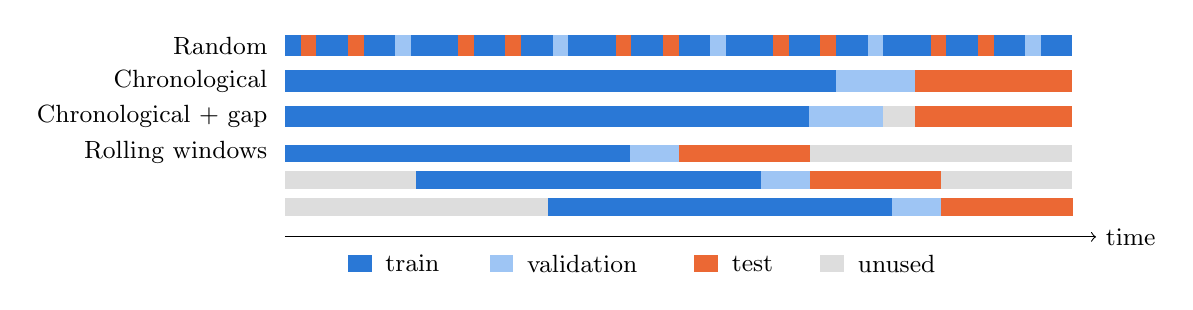
\begin{tikzpicture}[x=0.1cm,y=0.45cm,font=\small]
  \definecolor{tr}{HTML}{2A78D6}
  \definecolor{va}{HTML}{9EC5F4}
  \definecolor{te}{HTML}{EB6834}
  \definecolor{un}{HTML}{DDDDDD}
  % random: interleaved
  \node[anchor=east] at (-1,5.3) {Random};
  \foreach \i in {0,...,49} {
    \pgfmathsetmacro{\r}{mod(\i*7+3,10)}
    \pgfmathparse{\r<2 ? "te" : (\r<3 ? "va" : "tr")}
    \edef\c{\pgfmathresult}
    \fill[\c] (\i*2,5) rectangle ++(2,0.6);
  }
  % chronological
  \node[anchor=east] at (-1,4.3) {Chronological};
  \fill[tr] (0,4) rectangle (70,4.6); \fill[va] (70,4) rectangle (80,4.6); \fill[te] (80,4) rectangle (100,4.6);
  % gap
  \node[anchor=east] at (-1,3.3) {Chronological + gap};
  \fill[tr] (0,3) rectangle (66.5,3.6); \fill[va] (66.5,3) rectangle (76,3.6);
  \fill[un] (76,3) rectangle (80,3.6); \fill[te] (80,3) rectangle (100,3.6);
  % rolling
  \node[anchor=east] at (-1,2.3) {Rolling windows};
  \foreach \w in {0,1,2} {
    \pgfmathsetmacro{\y}{2-\w*0.75}
    \pgfmathsetmacro{\a}{\w*16.67}
    \fill[un] (0,\y) rectangle (100,\y+0.5);
    \fill[tr] (\a,\y) rectangle (\a+43.75,\y+0.5);
    \fill[va] (\a+43.75,\y) rectangle (\a+50,\y+0.5);
    \fill[te] (\a+50,\y) rectangle (\a+66.67,\y+0.5);
  }
  \draw[->] (0,-0.1) -- (103,-0.1) node[right] {time};
  % legend
  \begin{scope}[shift={(8,-1.1)}]
    \fill[tr] (0,0) rectangle (3,0.5); \node[anchor=west] at (3.5,0.25) {train};
    \fill[va] (18,0) rectangle (21,0.5); \node[anchor=west] at (21.5,0.25) {validation};
    \fill[te] (44,0) rectangle (47,0.5); \node[anchor=west] at (47.5,0.25) {test};
    \fill[un] (60,0) rectangle (63,0.5); \node[anchor=west] at (63.5,0.25) {unused};
  \end{scope}
\end{tikzpicture}
\caption{The split protocols. A random split interleaves training and test transactions in time, whereas the chronological protocols score only transactions that occur after every training transaction.}
\Description{Four horizontal bars over a time axis. In the random split, train, validation and test segments are interleaved. In the chronological split the first 70 percent is train, the next 10 percent validation and the last 20 percent test. The gap variant leaves the week before the test period unused. The rolling variant slides a train, validation and test window forward three times.}
\label{fig:splits}
\end{figure}


\begin{description}[leftmargin=1em,itemsep=2pt]
\item[Random.] A stratified random split into 70\% training, 10\% validation and 20\% test transactions (Figure~\ref{fig:splits}).
\item[Chronological.] Transactions are ordered by time. The first 70\% form the training set, the next 10\% the validation set and the last 20\% the test set.
\item[Chronological with a gap (IEEE-CIS).] As above, but the seven days before the test period are removed from the training and validation data. In production, the label of a transaction arrives only after a chargeback or an investigation, so the most recent transactions cannot be used for training~\cite{dalpozzolo2018credit}.
\item[Rolling windows (IEEE-CIS).] The six months are divided into six equal blocks. A model is trained on blocks $k$ to $k{+}2$ and tested on block $k{+}3$, for $k=1,2,3$. For each window we also draw a random split of the same four blocks with the same test-set size, so that the random-versus-chronological comparison is repeated on three different periods.
\end{description}

Under the random and chronological protocols, the final model is trained on the same number of transactions (80\%) and tested on the same number (20\%). The protocols differ only in \emph{which} transactions are assigned to each side.

The two test sets nevertheless differ, and a later period could simply be harder than an average one. We therefore add two controls in which both protocols are scored on the same transactions. The \emph{period-matched} control scores each random-split model only on those of its test transactions that fall inside the chronological test period. The \emph{blocked cross-validation} control compares five-fold cross-validation with random folds against five-fold cross-validation whose folds are five contiguous time blocks, so that each scheme tests every transaction exactly once. Blocked folds are not forward-looking, since a model may be trained on later data, but they remove the interleaving of training and test transactions in time, and the difference between the two schemes therefore isolates the effect of that interleaving.

\subsection{Models and tuning}

We evaluate five standard classifiers: logistic regression, a random forest~\cite{breiman2001random}, XGBoost~\cite{chen2016xgboost}, LightGBM~\cite{ke2017lightgbm} and a small multilayer perceptron (MLP). Table~\ref{tab:space} lists the search spaces.

Each model is tuned with 30 trials of Optuna's tree-structured Parzen estimator~\cite{akiba2019optuna}, maximizing \prauc{} on the validation set of the protocol at hand. The boosted models and the MLP use early stopping on validation \prauc{}. The selected configuration is then refitted on the combined training and validation data, with the number of boosting rounds or epochs found during tuning, and scored once on the test set. A seed repeats this entire pipeline, including the split (for the random protocol), tuning, refitting and testing, and we run five seeds. Under the chronological protocol the split is fixed, so the seeds vary only the tuner and the model. The standard deviations we report for that protocol therefore understate sampling uncertainty, and we complement them with a bootstrap over test transactions and with the rolling windows.

The tree models receive the raw matrix with missing values, and each tree of the random forest is grown on at most 100{,}000 sampled training rows. Logistic regression and the MLP receive median-imputed, standardized features with the amount log-transformed. The imputation and scaling statistics are computed on the training rows of each fit and never on validation or test rows.

\begin{table}[htbp]
\caption{Hyperparameter search spaces (30 trials per model, protocol and seed). $\alpha$ is the class-weight exponent of Section~\ref{sec:imbalance}.}
\label{tab:space}
\footnotesize
\begin{tabular}{ll}
\toprule
Model & Search space \\
\midrule
Logistic regression & $C \in [10^{-4}, 10^{2}]$ (log); $\alpha \in [0,1]$ \\
Random forest & 100 trees; depth $\in [4,24]$; minimum leaf size $\in [1,50]$ (log); feature fraction $\in [0.03,0.3]$; $\alpha$ \\
XGBoost & learning rate $\in [0.02,0.3]$ (log); depth $\in [3,10]$; minimum child weight $\in [1,50]$ (log); row \\
 & subsample $\in [0.5,1]$; column subsample $\in [0.3,1]$; $\lambda \in [10^{-2},10]$ (log); $\le$1000 rounds; $\alpha$ \\
LightGBM & learning rate $\in [0.02,0.3]$ (log); leaves $\in [15,255]$ (log); minimum leaf size $\in [10,200]$ (log); row \\
 & subsample $\in [0.5,1]$; column subsample $\in [0.3,1]$; $\lambda \in [10^{-2},10]$ (log); $\le$1000 rounds; $\alpha$ \\
MLP & 2--3 hidden layers of width 64, 128 or 256; dropout $\in [0,0.5]$; learning rate $\in [10^{-4},10^{-2}]$ (log); \\
 & weight decay $\in [10^{-6},10^{-3}]$ (log); AdamW, batch size 1024, $\le$30 epochs; $\alpha$ \\
\bottomrule
\end{tabular}
\end{table}

\subsection{Class imbalance and the oversampling leak}
\label{sec:imbalance}

The default treatment of class imbalance is cost-sensitive learning. The positive class receives weight $r^{\alpha}$, where $r$ is the ratio of legitimate to fraudulent training transactions and $\alpha \in [0,1]$ is tuned together with the other hyperparameters. A value of $\alpha=0$ corresponds to no weighting and $\alpha=1$ to full balancing.

A second experiment replaces class weights with SMOTE~\cite{chawla2002smote}, which synthesizes minority examples by interpolating between a minority example and one of its minority-class nearest neighbors. We run it in two ways under the random split.

\begin{description}[leftmargin=1em,itemsep=2pt]
\item[SMOTE on training rows.] The correct pipeline. Only the rows used to fit a model are oversampled, and validation and test rows are left untouched.
\item[SMOTE before the split.] The flawed pipeline described in some of the literature. The whole dataset is scaled and oversampled, and the balanced result is then split at random. Test rows are now half synthetic, and synthetic training rows have been interpolated from test fraud cases.
\end{description}

For the flawed pipeline we report two scores. The first is the score on its own oversampled test set, which is the number such a study would publish. The second is the score of the same fitted models on only the genuine transactions of that test set. The first score mixes two effects, a test set that no longer has the real class ratio and information flowing from test to training rows, whereas the second isolates the information flow.

On ULB the oversampling experiment uses the full data and five seeds. On IEEE-CIS, where oversampling doubles an already large training set, it uses a random subsample of 200{,}000 transactions and three seeds, with a class-weight baseline rerun on the same subsample. Rolling windows and cross-validation use one seed, since they already repeat the comparison over windows or folds.

\subsection{Metrics}

The primary metric is the area under the precision--recall curve (\prauc{}, computed as average precision), which is more informative than \rocauc{} when positives are rare~\cite{davis2006relationship,saito2015precision}. We also report \rocauc{} for comparison with prior work.

A fraud team can review only a limited number of alerts, so we additionally report \emph{alert-budget} metrics. The highest-scored 0.5\%, 1\% or 5\% of test transactions are flagged, and we measure \emph{recall}, the share of the test set's fraud cases that are flagged, and \emph{value recall}, the share of the fraudulent amount that the flagged transactions account for. Value recall weights each detected fraud case by its amount. The 5\% budget is included because fraud makes up more than 1\% of IEEE-CIS, which caps recall at the two smaller budgets.

\subsection{Implementation}

Experiments use Python 3.12 with scikit-learn 1.9~\cite{pedregosa2011scikit}, XGBoost 3.4, LightGBM 4.7, PyTorch 2.14~\cite{paszke2019pytorch}, imbalanced-learn 0.14 and Optuna 5.0, on a 14-core Apple M4 Pro laptop with 24\,GB of memory. The test scores of every run are stored, all tables and figures are generated from them, and code to reproduce every number is available at \ifanon a public repository (URL withheld for review)\else\url{https://github.com/mingwho/fraud-eval-time-aware}\fi.

\section{Results}
\label{sec:results}

\subsection{Random versus chronological split}

\begin{table}[t]
\caption{Random versus chronological split. Mean $\pm$ standard deviation over 5 seeds; $\Delta$ = chronological $-$ random.}
\label{tab:main}
\small
\begin{tabular}{llrrrrrr}
\toprule
 &  & \multicolumn{3}{c}{PR-AUC} & \multicolumn{3}{c}{ROC-AUC} \\
\cmidrule(lr){3-5}\cmidrule(lr){6-8}
Dataset & Model & Random & Chrono. & $\Delta$ & Random & Chrono. & $\Delta$ \\
\midrule
IEEE-CIS & Logistic regression & 0.474 {\scriptsize$\pm$ 0.006} & 0.360 {\scriptsize$\pm$ 0.001} & $-$0.114 & 0.865 {\scriptsize$\pm$ 0.005} & 0.840 {\scriptsize$\pm$ 0.001} & $-$0.025 \\
 & Random forest & 0.727 {\scriptsize$\pm$ 0.006} & 0.523 {\scriptsize$\pm$ 0.004} & $-$0.204 & 0.942 {\scriptsize$\pm$ 0.003} & 0.900 {\scriptsize$\pm$ 0.001} & $-$0.042 \\
 & XGBoost & 0.864 {\scriptsize$\pm$ 0.006} & 0.594 {\scriptsize$\pm$ 0.003} & $-$0.270 & 0.972 {\scriptsize$\pm$ 0.002} & 0.916 {\scriptsize$\pm$ 0.004} & $-$0.056 \\
 & LightGBM & 0.866 {\scriptsize$\pm$ 0.006} & 0.596 {\scriptsize$\pm$ 0.003} & $-$0.270 & 0.973 {\scriptsize$\pm$ 0.002} & 0.922 {\scriptsize$\pm$ 0.002} & $-$0.052 \\
 & MLP & 0.713 {\scriptsize$\pm$ 0.009} & 0.452 {\scriptsize$\pm$ 0.014} & $-$0.261 & 0.932 {\scriptsize$\pm$ 0.004} & 0.857 {\scriptsize$\pm$ 0.007} & $-$0.075 \\
\addlinespace
ULB & Logistic regression & 0.762 {\scriptsize$\pm$ 0.042} & 0.787 {\scriptsize$\pm$ 0.000} & $+$0.024 & 0.983 {\scriptsize$\pm$ 0.007} & 0.986 {\scriptsize$\pm$ 0.000} & $+$0.003 \\
 & Random forest & 0.851 {\scriptsize$\pm$ 0.023} & 0.797 {\scriptsize$\pm$ 0.010} & $-$0.055 & 0.980 {\scriptsize$\pm$ 0.004} & 0.980 {\scriptsize$\pm$ 0.010} & $+$0.000 \\
 & XGBoost & 0.856 {\scriptsize$\pm$ 0.036} & 0.796 {\scriptsize$\pm$ 0.013} & $-$0.059 & 0.986 {\scriptsize$\pm$ 0.006} & 0.984 {\scriptsize$\pm$ 0.004} & $-$0.002 \\
 & LightGBM & 0.859 {\scriptsize$\pm$ 0.027} & 0.781 {\scriptsize$\pm$ 0.018} & $-$0.078 & 0.983 {\scriptsize$\pm$ 0.006} & 0.974 {\scriptsize$\pm$ 0.025} & $-$0.009 \\
 & MLP & 0.845 {\scriptsize$\pm$ 0.016} & 0.811 {\scriptsize$\pm$ 0.013} & $-$0.034 & 0.977 {\scriptsize$\pm$ 0.006} & 0.986 {\scriptsize$\pm$ 0.004} & $+$0.009 \\
\bottomrule
\end{tabular}
\end{table}


\paragraph{IEEE-CIS}
Table~\ref{tab:main} gives the main comparison. Every model scores considerably lower when it is evaluated on later transactions. \prauc{} is lower by between \num{ieee.min.drop.pr} for logistic regression and \num{ieee.max.drop.pr} for the boosted models, which corresponds to \num{ieee.min.rel.pr}\% to \num{ieee.max.rel.pr}\% of the random-split score, and the mean difference over the five models is \num{ieee.mean.drop.pr}. These differences are far larger than the variation between seeds, and the bootstrap 95\% interval of the smallest one, for logistic regression, is [\num{ieee.lr.ci.lo}, \num{ieee.lr.ci.hi}].

\rocauc{} reflects the same effect but understates it. LightGBM moves from \num{ieee.lgbm.random.roc} to \num{ieee.lgbm.chrono.roc} on \rocauc{}, a change that would be easy to overlook in a results table, while its \prauc{} falls by about a third.

\paragraph{ULB}
On ULB, the three tree-based models lose \num{ulb.rf.drop.pr} to \num{ulb.lgbm.drop.pr} \prauc{} and their bootstrap intervals exclude zero. The MLP loses \num{ulb.mlp.drop.pr} with an interval of [\num{ulb.mlp.ci.lo}, \num{ulb.mlp.ci.hi}], and logistic regression shows no loss. Two caveats apply even to the tree-model result. The dataset is small, with \num{ulb.testfraud} fraud cases in the chronological test set, and the random-split score itself has a standard deviation of \num{ulb.rf.random.pr.sd} to \num{ulb.lr.random.pr.sd} across seeds, which is comparable to the differences between models that studies on this dataset report. In addition, as the next subsection shows, most of this drop is not attributable to leakage.

\paragraph{Model rankings}
On IEEE-CIS, the split does not change the order of the models (Kendall's $\tau=\num{ieee.tau.pr}$ between the two \prauc{} rankings), but it changes the distances between them. The spread between the best and the worst model shrinks from \num{ieee.range.random.pr} to \num{ieee.range.chrono.pr}. On ULB, the random split ranks the tree ensembles well ahead of logistic regression, whereas under the chronological split all five models fall within \num{ulb.range.chrono.pr} of each other and the order changes ($\tau=\num{ulb.tau.pr}$). Given the noise on ULB, we interpret this as the absence of a detectable difference between models rather than as a new ranking.

\subsection{Is the later period simply harder?}
\label{sec:controls}

A lower score on the last 20\% of the timeline could indicate that those weeks are harder, rather than that the random split leaked information. Table~\ref{tab:controls} reports the two controls that score both protocols on the same transactions.

\begin{table}[t]
\caption{Controls that score both protocols on the same transactions (\prauc{}). Left: random-split models scored only on their test transactions inside the chronological test period, against the chronological models. Right: five-fold cross-validation with random folds against contiguous time blocks.}
\label{tab:controls}
\small
\begin{tabular}{llrrrrrr}
\toprule
 & & \multicolumn{3}{c}{Same test period} & \multicolumn{3}{c}{Five-fold cross-validation} \\
\cmidrule(lr){3-5}\cmidrule(lr){6-8}
Dataset & Model & Random & Chrono. & $\Delta$ & Random folds & Time blocks & $\Delta$ \\
\midrule
IEEE-CIS & Logistic regression & 0.432 & 0.360 & $-$0.072 & 0.469 & 0.410 & $-$0.059 \\
 & Random forest & 0.725 & 0.523 & $-$0.202 & -- & -- & -- \\
 & XGBoost & 0.871 & 0.594 & $-$0.277 & -- & -- & -- \\
 & LightGBM & 0.870 & 0.598 & $-$0.273 & -- & -- & -- \\
 & MLP & 0.714 & 0.452 & $-$0.262 & 0.710 & 0.495 & $-$0.214 \\
\addlinespace
ULB & Logistic regression & 0.762 & 0.787 & $+$0.024 & 0.752 & 0.775 & $+$0.023 \\
 & Random forest & 0.771 & 0.797 & $+$0.026 & 0.850 & 0.790 & $-$0.060 \\
 & XGBoost & 0.765 & 0.796 & $+$0.031 & 0.853 & 0.792 & $-$0.061 \\
 & LightGBM & 0.753 & 0.781 & $+$0.028 & 0.846 & 0.787 & $-$0.059 \\
 & MLP & 0.775 & 0.811 & $+$0.036 & -- & -- & -- \\
\bottomrule
\end{tabular}
\end{table}


\paragraph{IEEE-CIS}
Restricting the random-split models to the test transactions that fall inside the chronological test period, about \num{ieee.matched.nfraud} fraud cases per seed, leaves their scores essentially unchanged for four of the five models. The random forest scores \num{ieee.rf.matched.pr} on that period compared with \num{ieee.rf.random.pr} overall, and LightGBM scores \num{ieee.lgbm.matched.pr} compared with \num{ieee.lgbm.random.pr}. The period is therefore not harder for these models, and what they lose under the chronological split is consistent with the benefit of having trained on transactions from the same weeks. Logistic regression is the exception. It scores \num{ieee.lr.matched.pr} on that period, so about a third of its drop reflects a harder period and two thirds the split. The cross-validation control agrees with this picture. With every transaction tested exactly once under both schemes, contiguous time blocks give lower \prauc{} than random folds for every model, and when averaged over the models the difference is positive in each of the five blocks (\num{ieee.blocks.mindrop} to \num{ieee.blocks.maxdrop}).

\paragraph{ULB}
On ULB, the controls lead to a different conclusion. Scored only on the final period, the random-split models do no better than the chronological ones, and in fact score slightly lower for all five models, although with about \num{ulb.matched.nfraud} fraud cases per seed the estimate is noisy. The drop in Table~\ref{tab:main} is therefore largely attributable to a harder final period. Cross-validation shows that interleaving does help the non-linear models on ULB, by 0.06 to 0.07 on average, but the benefit is uneven across the two days. Averaged over the models, it is \num{ulb.block1.drop} in the first of the five time blocks, \num{ulb.block3.drop} and \num{ulb.block4.drop} in the third and fourth, and absent in the second (\num{ulb.block2.drop}) and in the fifth (\num{ulb.block5.drop}), the fifth being the block that a chronological split tests. The controls are therefore necessary for interpreting the ULB result, and two days of data with \num{ulb.fraud} fraud cases do not support stronger conclusions.

\subsection{Different periods, label delay and time since training}

\begin{figure}[htbp]
\centering
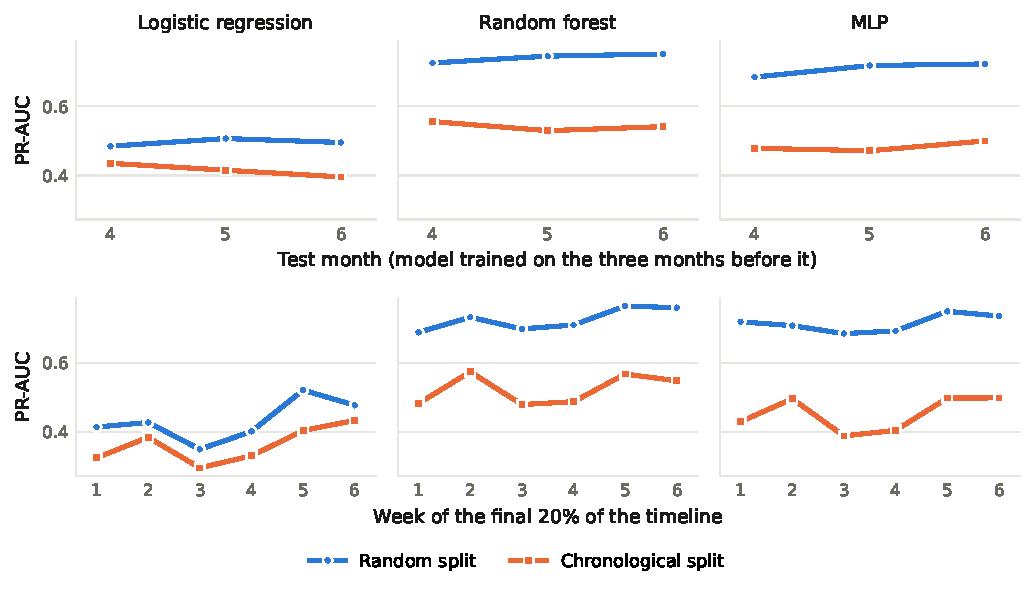
\includegraphics[width=\linewidth]{generated/fig_time.pdf}
\caption{IEEE-CIS. Top: \prauc{} on each rolling window, for a model trained on the three preceding months and for a random split of the same four months. Bottom: \prauc{} of the main-comparison models on each week of the final 20\% of the timeline, where random-split models are scored on their test transactions from that week.}
\Description{Two rows of five small line charts, one column per model. In every panel the random-split line lies above the chronological line. In the top row both lines are roughly flat across test months four to six. In the bottom row both lines move together across six weeks and the distance between them stays about the same.}
\label{fig:time}
\end{figure}

The top row of Figure~\ref{fig:time} repeats the comparison on three different four-month windows of IEEE-CIS. The random split scores higher than the chronological one for every model in every window, with differences ranging from \num{ieee.roll.mindrop} to \num{ieee.roll.maxdrop} and averaging \num{ieee.roll.meandrop}.

Removing the last seven days before the test period from the training data, to mimic label delay, has a small additional cost. Depending on the model, \prauc{} falls by a further \num{ieee.min.gap7.drop} to \num{ieee.max.gap7.drop}.

The bottom row of Figure~\ref{fig:time} follows the models through the six weeks of the test period. If the gap were caused by gradual drift, the chronological models would start close to the random-split ones and fall away over time. Instead, the gap is already close to its full size in the first week after the training cut-off, and over the six weeks it fluctuates and widens only slightly for the boosted models. The two curves rise and fall together, which reflects weeks that are easier or harder for any model. The advantage conferred by the random split is therefore lost as soon as training and test transactions are no longer interleaved (Section~\ref{sec:mechanism}).

\subsection{Alert budgets}

\begin{table}[t]
\caption{Alert-budget metrics under the two splits: share of fraud cases (recall) and of fraud value caught when the highest-scored 0.5\% or 1\% of test transactions are flagged.}
\label{tab:budget}
\small
\begin{tabular}{llrrrrrrrrr}
\toprule
 &  & \multicolumn{3}{c}{Recall at 0.5\% budget} & \multicolumn{3}{c}{Recall at 1\% budget} & \multicolumn{3}{c}{Value recall at 1\% budget} \\
\cmidrule(lr){3-5}\cmidrule(lr){6-8}\cmidrule(lr){9-11}
Dataset & Model & Random & Chrono. & $\Delta$ & Random & Chrono. & $\Delta$ & Random & Chrono. & $\Delta$ \\
\midrule
IEEE-CIS & Logistic regression & 0.138 {\scriptsize$\pm$ 0.001} & 0.110 {\scriptsize$\pm$ 0.001} & -0.027 & 0.249 {\scriptsize$\pm$ 0.003} & 0.197 {\scriptsize$\pm$ 0.001} & -0.052 & 0.164 {\scriptsize$\pm$ 0.007} & 0.133 {\scriptsize$\pm$ 0.001} & -0.031 \\
 & Random forest & -- & -- & -- & -- & -- & -- & -- & -- & -- \\
 & XGBoost & -- & -- & -- & -- & -- & -- & -- & -- & -- \\
 & LightGBM & -- & -- & -- & -- & -- & -- & -- & -- & -- \\
 & MLP & 0.143 {\scriptsize$\pm$ 0.000} & 0.133 {\scriptsize$\pm$ 0.001} & -0.010 & 0.283 {\scriptsize$\pm$ 0.000} & 0.235 {\scriptsize$\pm$ 0.003} & -0.049 & 0.214 {\scriptsize$\pm$ 0.009} & 0.163 {\scriptsize$\pm$ 0.002} & -0.051 \\
\addlinespace
ULB & Logistic regression & 0.878 {\scriptsize$\pm$ 0.028} & 0.867 {\scriptsize$\pm$ 0.000} & -0.011 & 0.890 {\scriptsize$\pm$ 0.026} & 0.875 {\scriptsize$\pm$ 0.007} & -0.015 & 0.763 {\scriptsize$\pm$ 0.065} & 0.695 {\scriptsize$\pm$ 0.001} & -0.068 \\
 & Random forest & 0.878 {\scriptsize$\pm$ 0.029} & 0.832 {\scriptsize$\pm$ 0.031} & -0.046 & 0.890 {\scriptsize$\pm$ 0.028} & 0.856 {\scriptsize$\pm$ 0.026} & -0.034 & 0.773 {\scriptsize$\pm$ 0.083} & 0.737 {\scriptsize$\pm$ 0.053} & -0.036 \\
 & XGBoost & 0.882 {\scriptsize$\pm$ 0.025} & 0.819 {\scriptsize$\pm$ 0.007} & -0.063 & 0.906 {\scriptsize$\pm$ 0.023} & 0.853 {\scriptsize$\pm$ 0.019} & -0.053 & 0.821 {\scriptsize$\pm$ 0.108} & 0.779 {\scriptsize$\pm$ 0.027} & -0.043 \\
 & LightGBM & 0.880 {\scriptsize$\pm$ 0.023} & 0.824 {\scriptsize$\pm$ 0.030} & -0.056 & 0.892 {\scriptsize$\pm$ 0.015} & 0.853 {\scriptsize$\pm$ 0.025} & -0.039 & 0.767 {\scriptsize$\pm$ 0.056} & 0.794 {\scriptsize$\pm$ 0.061} & +0.027 \\
 & MLP & 0.882 {\scriptsize$\pm$ 0.019} & 0.861 {\scriptsize$\pm$ 0.015} & -0.020 & 0.898 {\scriptsize$\pm$ 0.020} & 0.883 {\scriptsize$\pm$ 0.011} & -0.015 & 0.788 {\scriptsize$\pm$ 0.044} & 0.835 {\scriptsize$\pm$ 0.081} & +0.047 \\
\bottomrule
\end{tabular}
\end{table}


Table~\ref{tab:budget} translates the comparison into review workload. On IEEE-CIS, fraud accounts for \num{ieee.rate}\% of transactions, so a 0.5\% or 1\% budget is smaller than the fraud volume and recall is capped. Within that cap, the top of the ranking holds up comparatively well. At a 1\% budget, the precision of LightGBM's alerts is \num{ieee.lgbm.random.p01} under the random split and \num{ieee.lgbm.chrono.p01} under the chronological one, although for logistic regression and the MLP it falls to \num{ieee.lr.chrono.p01} and \num{ieee.mlp.chrono.p01}. The inflation is concentrated deeper in the ranking. At a 5\% budget, which is large enough to contain every fraud case, LightGBM catches \num{ieee.lgbm.random.r05} of fraud cases and \num{ieee.lgbm.random.v05} of fraud value under the random split, but \num{ieee.lgbm.chrono.r05} and \num{ieee.lgbm.chrono.v05} on future transactions.

On IEEE-CIS, value recall is lower than recall for every model at the 1\% budget, because the fraud cases that are easiest to rank at the top are smaller than average, so counting cases overstates the value protected. On ULB, the alert-budget metrics change little, consistent with Section~\ref{sec:controls}.

\subsection{Oversampling before the split}

\begin{table}[t]
\caption{Oversampling leak under a random split. ``As reported'' scores the flawed pipeline on its own oversampled test set; ``genuine test rows'' scores the same models on the genuine transactions of that test set. Mean over 5 seeds.}
\label{tab:smote}
\small
\begin{tabular}{llrrrrrrrr}
\toprule
 &  & \multicolumn{2}{c}{\shortstack{Class\\weights}} & \multicolumn{2}{c}{\shortstack{SMOTE on\\training rows}} & \multicolumn{2}{c}{\shortstack{SMOTE before split,\\as reported}} & \multicolumn{2}{c}{\shortstack{SMOTE before split,\\genuine test rows}} \\
\cmidrule(lr){3-4}\cmidrule(lr){5-6}\cmidrule(lr){7-8}\cmidrule(lr){9-10}
Dataset & Model & PR-AUC & F1 & PR-AUC & F1 & PR-AUC & F1 & PR-AUC & F1 \\
\midrule
IEEE-CIS & Logistic regression & 0.476 & 0.442 & 0.449 & 0.234 & 0.891 & 0.789 & 0.456 & 0.241 \\
 & Random forest & 0.677 & 0.629 & 0.598 & 0.578 & 0.998 & 0.985 & 0.751 & 0.698 \\
 & XGBoost & -- & -- & -- & -- & -- & -- & -- & -- \\
 & LightGBM & -- & -- & -- & -- & -- & -- & -- & -- \\
 & MLP & 0.606 & 0.589 & 0.563 & 0.448 & 0.998 & 0.986 & 0.926 & 0.797 \\
\addlinespace
ULB & Logistic regression & 0.762 & 0.776 & 0.761 & 0.110 & 0.990 & 0.943 & 0.742 & 0.112 \\
 & Random forest & 0.851 & 0.851 & 0.856 & 0.718 & 1.000 & 1.000 & 0.986 & 0.855 \\
 & XGBoost & 0.856 & 0.854 & 0.867 & 0.787 & 1.000 & 1.000 & 0.994 & 0.898 \\
 & LightGBM & 0.859 & 0.856 & 0.854 & 0.729 & 1.000 & 1.000 & 0.890 & 0.846 \\
 & MLP & 0.845 & 0.768 & 0.835 & 0.790 & 1.000 & 1.000 & 0.991 & 0.876 \\
\bottomrule
\end{tabular}
\end{table}


Table~\ref{tab:smote} shows the second leak. Applied to the whole dataset before a random split, SMOTE produces the near-perfect figures familiar from the literature. On its own oversampled test set, the flawed pipeline reports a \prauc{} of \num{ulb.min.leakrep.pr} or more for every model on ULB and between \num{ieee.min.leakrep.pr} and \num{ieee.max.leakrep.pr} on IEEE-CIS, with correspondingly high F1 scores.

Part of this is an artifact of the test set, which is half synthetic fraud and no longer has the real class ratio. Scoring the same fitted models on only the genuine test transactions indicates, however, that real information has leaked as well. On ULB, XGBoost reaches \num{ulb.xgb.leakreal.pr}, the random forest \num{ulb.rf.leakreal.pr} and the MLP \num{ulb.mlp.leakreal.pr} on genuine transactions, compared with \num{ulb.xgb.smote.pr}, \num{ulb.rf.smote.pr} and \num{ulb.mlp.smote.pr} when only the training rows are oversampled. On IEEE-CIS, the MLP goes from \num{ieee.mlp.smote.pr} to \num{ieee.mlp.leakreal.pr} and the random forest from \num{ieee.rf.smote.pr} to \num{ieee.rf.leakreal.pr}, while the boosted models gain less (\num{ieee.lgbm.smote.pr} to \num{ieee.lgbm.leakreal.pr} for LightGBM). The mechanism is that a synthetic training point is placed on the segment between a fraud case and one of its neighbors, so that when the fraud case is assigned to the test set, the training set contains points immediately next to it that are labeled as fraud.

Logistic regression shows no measurable benefit from the leak on either dataset (\num{ulb.lr.leakreal.pr} compared with \num{ulb.lr.smote.pr} on ULB), which is what one would expect of a linear boundary that cannot exploit a small number of local points. The leak thus behaves like a memorization effect. It is not detectable for the linear model and is present, in varying size, for every non-linear one. LightGBM on ULB reaches 0.98 or more in four of five seeds, and in the fifth its training diverged, which reduces the mean to \num{ulb.lgbm.leakreal.pr}.

A secondary result is that SMOTE applied correctly does not improve on tuned class weights. On IEEE-CIS it is worse for every model (mean \prauc{} \num{ieee.mean.smote.pr} compared with \num{ieee.mean.weight.pr}), and on ULB the two are indistinguishable (\num{ulb.mean.smote.pr} compared with \num{ulb.mean.weight.pr}).

\subsection{Where the inflation comes from}
\label{sec:mechanism}

Fraud is not spread evenly over cards or over time, and a random split places parts of the same fraud episode on both sides of the split.

For IEEE-CIS, we constructed a proxy for a payment card from the card and address columns and the day on which the card was first seen. Among cards with more than one transaction, 97\% carry a single label throughout, so knowing that a card was fraudulent once is almost as informative as knowing the label. Under a random split, \num{ieee.key.fraud.random}\% of the fraud cases in the test set belong to a card that also has a fraud case in the training data. Under the chronological split the figure is \num{ieee.key.fraud.chrono}\%, and with the seven-day gap it is \num{ieee.key.fraud.chrono_gap}\%. For legitimate test transactions, the corresponding figures are \num{ieee.key.legit.random}\% and \num{ieee.key.legit.chrono}\%. A model that has learned to recognize previously flagged cards is therefore rewarded about three times as often under the random split, and no single column needs to identify the card, since a flexible model can in principle recover it from a combination of columns. This also accounts for the shape of the weekly curves in Figure~\ref{fig:time}. The advantage is consistent with access to other transactions of the same fraud episode, including later ones. Under a random split these are available for most episodes, whereas under a chronological split only the earlier transactions of episodes that began before the cut-off are available.

ULB has no card columns, but the same clustering is visible in time. Under a random split, \num{ulb.prox.min1.random}\% of test fraud cases have a training fraud case within one minute, \num{ulb.prox.min10.random}\% have one within ten minutes, and \num{ulb.prox.dup.random}\% are exact duplicates of a training fraud case in all features. Under the chronological split, no test fraud case has a training fraud case within ten minutes, and none is a duplicate of one.

Giving the models the raw timestamp as a feature made no measurable difference on ULB. The mean random-split \prauc{} is \num{ulb.mean.tf.random} with the timestamp and \num{ulb.mean.random.pr} without it.

\section{Discussion}
\label{sec:discussion}

\paragraph{What the random split measures}
The results are consistent with a single explanation. Fraud occurs in episodes, in which a compromised card is used several times within minutes or days and the transactions of an episode resemble each other. A random split distributes each episode over the training and test data, so the test measures whether a model can recognize the remainder of an episode that it has already seen labeled. This task is much easier than detecting a new episode, and a random split additionally provides the model with every other transaction of the episode, including later ones. The chronological split poses the question that a deployed system faces. The difference between the two is not primarily gradual concept drift, which would grow with the distance from the training period, because nearly all of it is present in the first week.

The size of the gap depends on how much a model can memorize. Logistic regression loses the least in absolute terms on IEEE-CIS and shows no measurable loss from the oversampling leak, whereas the tree ensembles and the MLP lose the most. A random split therefore overstates performance and also overstates the benefit of model capacity.

\paragraph{What the two datasets can support}
IEEE-CIS is large enough for these effects to be measured precisely, but ULB is not. Its \num{ulb.fraud} fraud cases over two days leave a chronological test set of \num{ulb.testfraud} cases and random-split scores that vary by several points from seed to seed, so an improvement of a point or two of \prauc{} on a single split of ULB lies within the noise, whereas the oversampling leak is far larger than the noise.

\paragraph{A checklist for evaluating fraud models}
\begin{enumerate}[leftmargin=1.8em,itemsep=2pt]
\item \textbf{Split by time.} Train on earlier transactions and test on later ones, and state the cut points. Tune on a validation period that lies between them.
\item \textbf{Respect label delay.} Leave a gap between training and test periods that matches the time labels take to arrive.
\item \textbf{Fit all preprocessing on training rows only.} This includes imputation, scaling, encoding, feature selection and resampling. Resample after splitting, and never resample the test set.
\item \textbf{Score at the real class ratio.} Report \prauc{} and recall at a stated alert budget on unmodified test data. Accuracy and F1 on a rebalanced test set are not informative.
\item \textbf{Check that a gap is leakage.} A later period can be harder. Compare protocols on the same transactions, as in Section~\ref{sec:controls}, before attributing a difference to the split.
\item \textbf{Repeat over periods and report variance.} Use rolling windows where the data allow it. On small datasets, state how many fraud cases the test set contains and how much the score varies across splits.
\item \textbf{Report value-weighted metrics.} Recall by value can differ from recall by count.
\item \textbf{Release code and stored predictions,} so that others can recompute metrics under a different protocol.
\end{enumerate}

\paragraph{Limitations}
Both datasets are public and anonymized, and we deliberately used raw features. A production system would add card-history aggregates, which change both the level of performance and possibly the size of the gap, so our numbers are not estimates of production performance. The card key we use on IEEE-CIS is a heuristic, and we do not know how or when that dataset's labels were assigned. For reasons of cost, the IEEE-CIS oversampling experiment used a 200{,}000-transaction subsample with three seeds, and the rolling windows and cross-validation used one seed. The chronological protocols score a fixed model on six weeks of data and do not model retraining or investigator feedback, which the realistic-evaluation literature treats in depth~\cite{dalpozzolo2018credit}.

\ifanon\else
\begin{acks}
In preparing this paper, the authors used Claude Code (Anthropic) as a coding and writing assistant. We used it to implement the experiment pipeline, run the experiments, produce drafts of the text, and check references. We designed the study, specified the experiments and the analyses, reviewed and edited all code, results and text, and take full responsibility for the content.
\end{acks}
\fi

\section{Conclusion}

On the larger of the two public payment-fraud datasets, the \prauc{} of five standard classifiers is \num{ieee.min.rel.pr}--\num{ieee.max.rel.pr}\% lower on future transactions than a random split suggests, and oversampling before the split inflates scores further. The results suggest that overlap between fraud episodes in the training and test data is an important contributor to this inflation in both cases. On the smaller dataset, the split matters less than it first appears and the oversampling leak matters more, and the dataset is too small to support the fine-grained model comparisons that are often drawn from a single split of it. Time-ordered splits, resampling confined to the training data, alert-budget metrics and a comparison on the same transactions are inexpensive to adopt, and they make a benchmark score a closer estimate of the performance a fraud team would observe.


\bibliographystyle{ACM-Reference-Format}
\bibliography{refs}

\end{document}
